\section{Diagramas de casos de uso}
\label{sec:casos_uso}

    Los diagramas de casos de uso bajo el estándar UML 2.5 formalizan los límites del sistema, identificando quién ejecuta cada acción y qué subsistemas intervienen. La herramienta PlantUML permitió generar estas representaciones a partir de código fuente.

    Reunir ochenta y seis casos de uso en un único diagrama saturaría la página A4 y destruiría la legibilidad del documento. Por este motivo, el sistema se divide en nueve paquetes temáticos. Antes de descender al detalle de cada paquete, resulta necesario definir los actores que intervienen en la aplicación.

\subsection{Actores del sistema}

    El modelo contempla usuarios humanos (con roles que varían según el contexto de la vivienda) y servicios externos integrados mediante APIs seguras. La figura \ref{fig:jerarquia_actores} representa las relaciones de generalización y herencia entre ellos.

\begin{figure}[H]
    \centering
    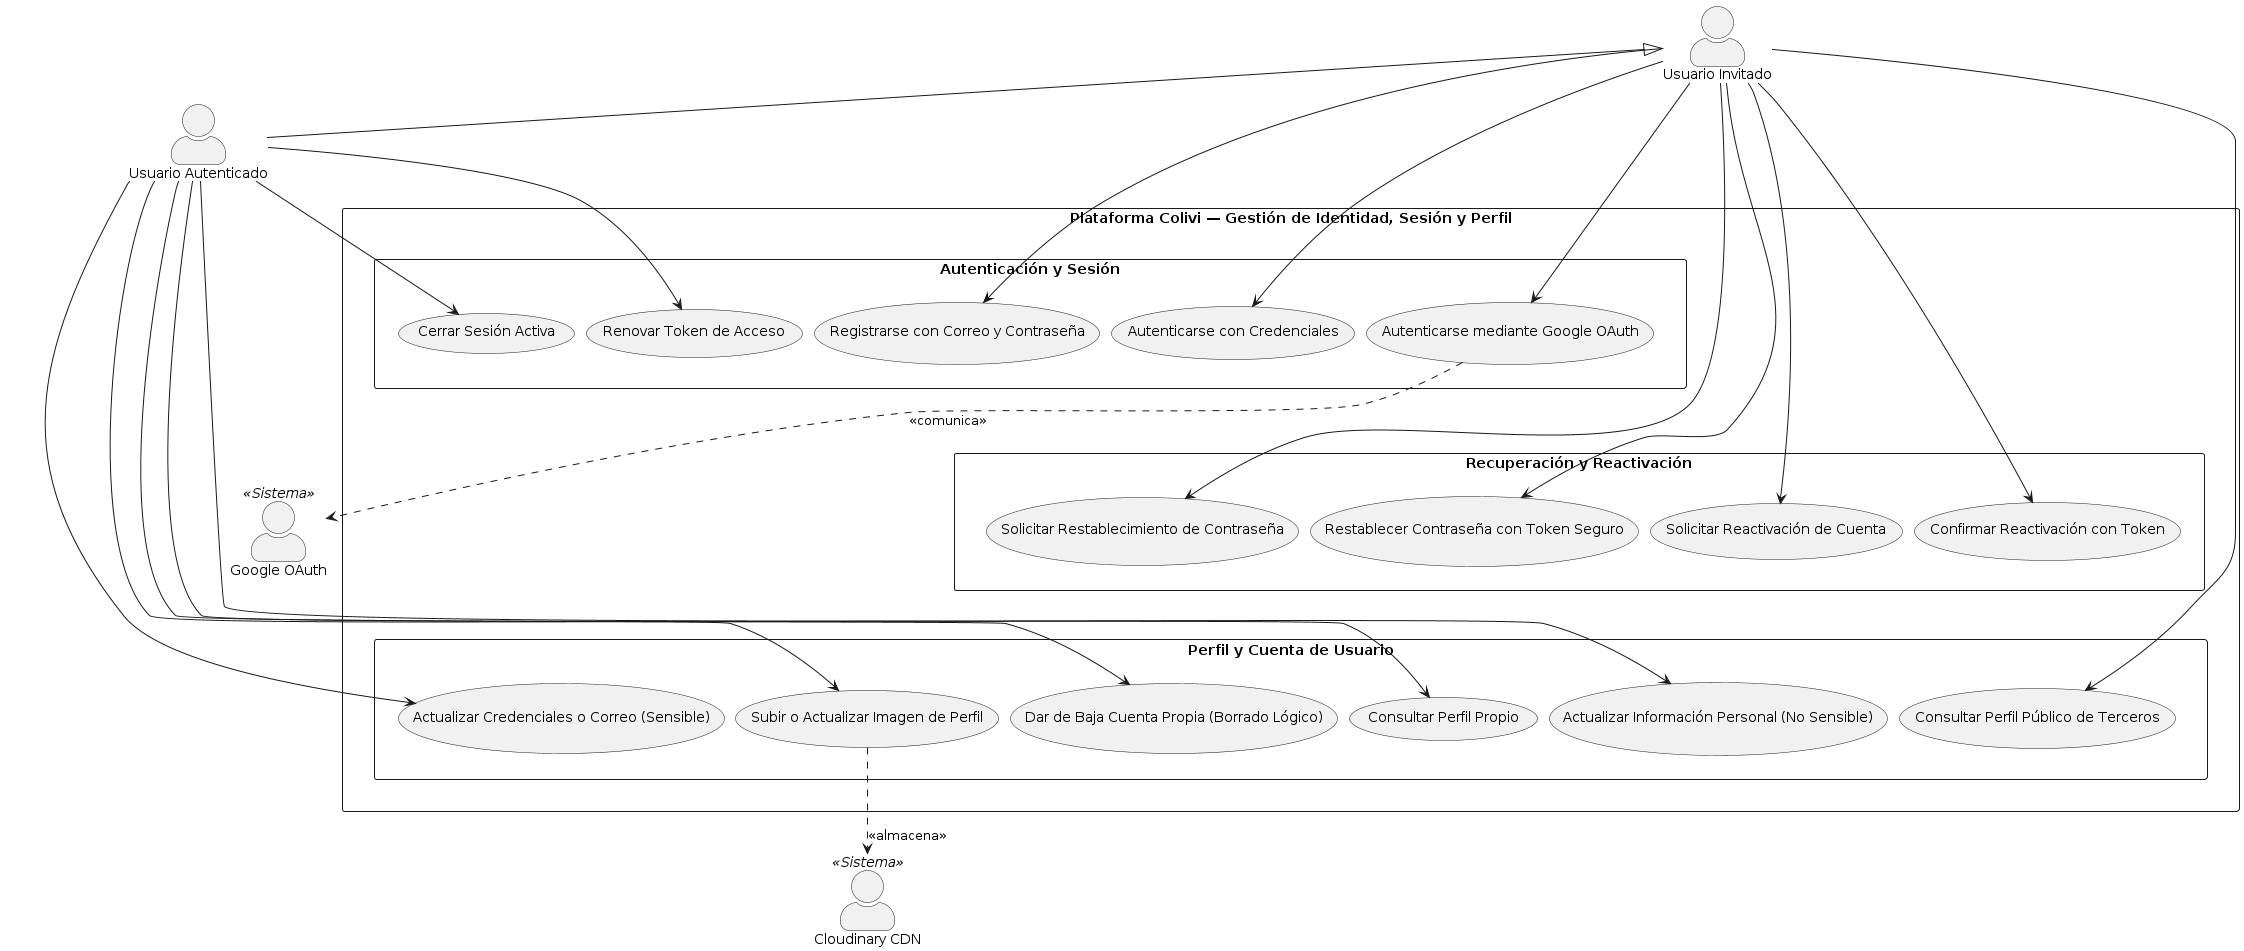
\includegraphics[width=0.68\textwidth]{AnalisisFuncional/img/jerarquia_actores.png}
    \caption{Jerarquía y relaciones de herencia entre los actores del sistema. Elaboración propia}
    \label{fig:jerarquia_actores}
\end{figure}

    Cada actor asume un rol delimitado en la aplicación:

\begin{itemize}
    \item \textbf{Usuario Invitado}: navega de forma anónima sin sesión abierta. Explora el mapa de inmuebles, consulta fichas de habitaciones y solicita el registro o inicio de sesión.
    \item \textbf{Usuario Autenticado}: dispone de un token JWT válido. Gestiona sus datos de perfil, abre conversaciones en el chat, envía denuncias a moderación y formula preguntas al asistente virtual.
    \item \textbf{Inquilino}: usuario autenticado que busca piso. Emite solicitudes de reserva acotadas en el calendario, abona depósitos de fianza y puntúa las estancias finalizadas.
    \item \textbf{Anfitrión}: usuario autenticado que oferta propiedades. Da de alta inmuebles, publica anuncios con sus características físicas, administra la galería de fotos y acepta o declina solicitudes de reserva.
    \item \textbf{Compañero de Piso}: miembro integrado en un piso activo. Registra gastos comunes, revisa balances de deuda, transfiere liquidaciones y marca tareas de limpieza como completadas.
    \item \textbf{Administrador del Hogar}: compañero de piso responsable de coordinar la vivienda. Genera invitaciones efímeras, expulsa a residentes sin deudas pendientes y programa las tareas recurrentes.
    \item \textbf{Administrador del Sistema}: superusuario con permisos globales de moderación. Examina la cola de denuncias, audita conversaciones notificadas y bloquea cuentas o anuncios fraudulentos.
    \item \textbf{Google OAuth}: proveedor de identidad que expide credenciales federadas para agilizar el acceso sin contraseña local.
    \item \textbf{Cloudinary CDN}: infraestructura externa encargada de almacenar, transformar y servir imágenes de anuncios y avatares de usuario.
    \item \textbf{OpenStreetMap / Nominatim}: motor cartográfico consumido por el cliente web para transformar direcciones postales en coordenadas geográficas de latitud y longitud.
\end{itemize}

\subsection{Especificación detallada de casos de uso}

    Cada caso de uso se especifica mediante una ficha estructurada que define su código identificador, el actor detonante, las precondiciones del dominio, la descripción funcional y el flujo secuencial de interacción entre el usuario y la plataforma.

\subsection{Paquete 1: Gestión de identidad, sesión y perfil}

    El paquete centraliza el registro de cuentas, la expedición y rotación de tókenes de seguridad, el restablecimiento de contraseñas y el ciclo de vida del perfil. La figura \ref{fig:dcu_identidad} representa las relaciones entre los actores y los quince casos de uso del módulo.

\begin{figure}[H]
    \centering
    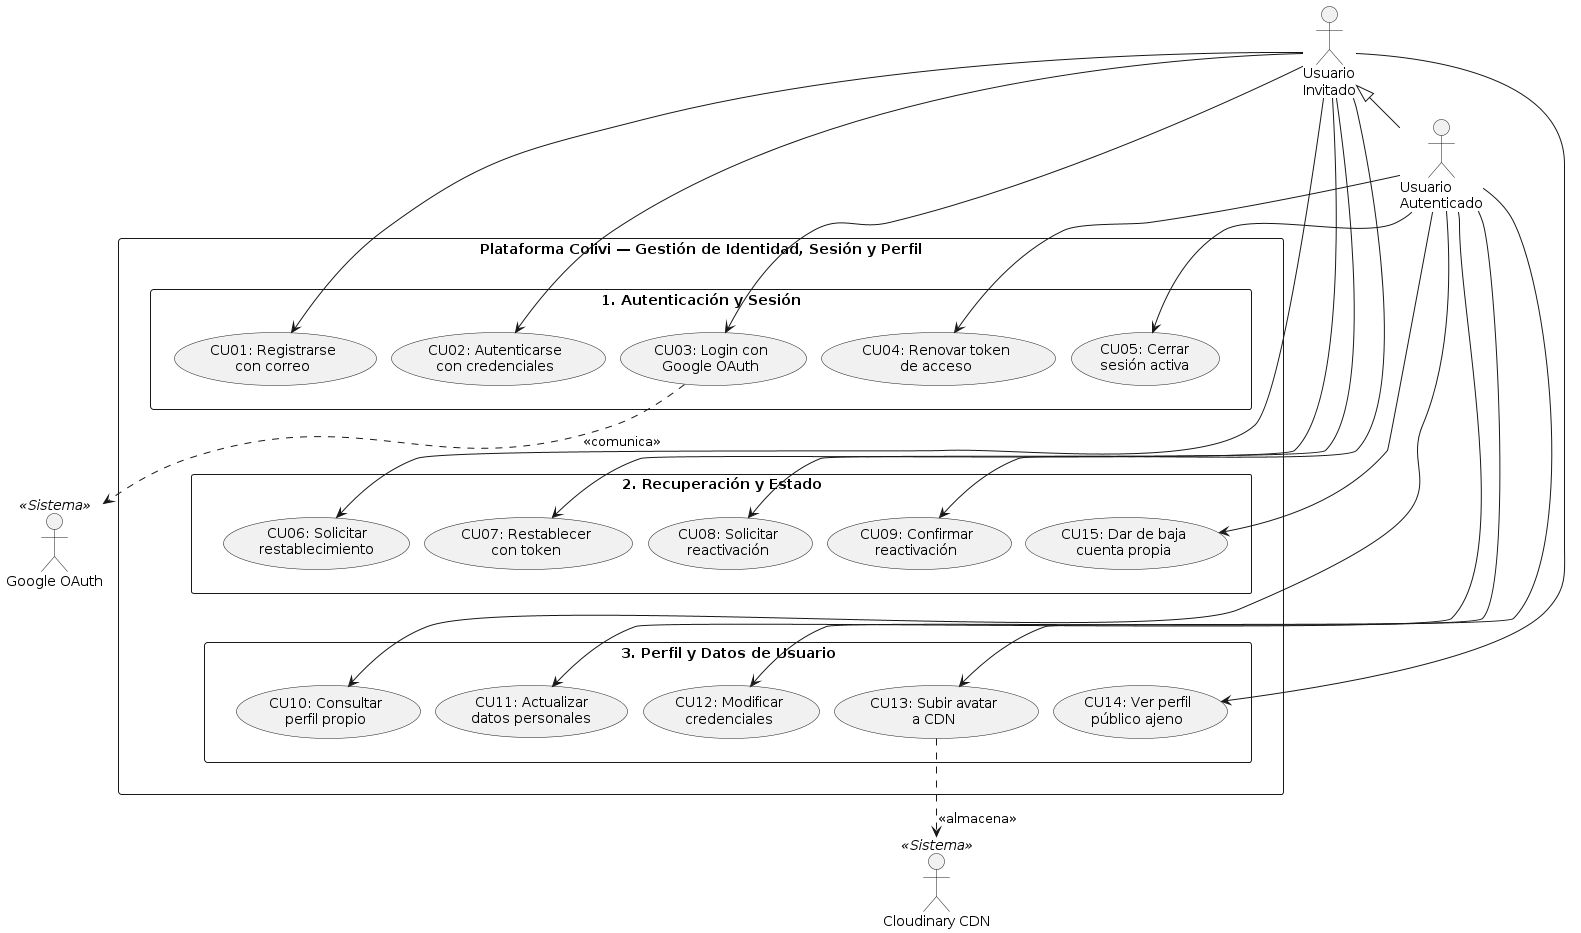
\includegraphics[width=0.95\textwidth]{AnalisisFuncional/img/dcu_identidad.png}
    \caption{Diagrama de casos de uso del módulo de identidad, sesión y perfil}
    \label{fig:dcu_identidad}
\end{figure}

    Las siguientes tablas recogen la especificación formal de cada caso de uso:

\begin{table}[H]
\centering
\begin{tabular}{|p{3.1cm}|p{10.9cm}|}
\hline
\textbf{Caso de Uso} & \textbf{CU01: Registrarse con correo y contraseña} \\ \hline
\textbf{Actores} & Usuario Invitado \\ \hline
\textbf{Descripción} & Permite a un nuevo usuario crear una cuenta local mediante credenciales \\ \hline
\textbf{Precondiciones} & No poseer una sesión activa y que el correo no figure previamente registrado \\ \hline
\textbf{Flujo básico} & 
1. El usuario accede al formulario de registro en la interfaz de usuario. \newline
2. El usuario introduce nombre, apellidos, dirección de correo electrónico y contraseña. \newline
3. El sistema valida el formato de los datos y comprueba la disponibilidad del correo. \newline
4. El sistema almacena la credencial protegida con un algoritmo de dispersión criptográfica y confirma la creación de la cuenta. \\ \hline
\end{tabular}
\caption{Especificación del caso de uso CU01.}
\label{tab:cu01}
\end{table}

\begin{table}[H]
\centering
\begin{tabular}{|p{3.1cm}|p{10.9cm}|}
\hline
\textbf{Caso de Uso} & \textbf{CU02: Autenticarse con credenciales} \\ \hline
\textbf{Actores} & Usuario Invitado \\ \hline
\textbf{Descripción} & Valida las credenciales locales para expedir una sesión sin estado \\ \hline
\textbf{Precondiciones} & Estar registrado y que la cuenta no se encuentre dada de baja o suspendida \\ \hline
\textbf{Flujo básico} & 
1. El usuario accede a la vista de inicio de sesión e introduce correo y contraseña. \newline
2. El sistema valida la coincidencia de las credenciales frente a la base de datos. \newline
3. El sistema genera un par de tókenes JWT (acceso y renovación) con los roles asignados. \newline
4. El cliente almacena los tókenes de manera segura y redirige al panel principal. \\ \hline
\end{tabular}
\caption{Especificación del caso de uso CU02.}
\label{tab:cu02}
\end{table}

\begin{table}[H]
\centering
\begin{tabular}{|p{3.1cm}|p{10.9cm}|}
\hline
\textbf{Caso de Uso} & \textbf{CU03: Autenticarse mediante Google OAuth} \\ \hline
\textbf{Actores} & Usuario Invitado, Google OAuth \\ \hline
\textbf{Descripción} & Permite iniciar sesión o registrarse mediante delegación de identidad federada \\ \hline
\textbf{Precondiciones} & Poseer una cuenta activa y verificada en el proveedor Google \\ \hline
\textbf{Flujo básico} & 
1. El usuario pulsa sobre la opción de acceso con Google en la interfaz. \newline
2. El proveedor solicita el consentimiento y devuelve un token de identidad criptográfico. \newline
3. El backend verifica la autenticidad del token frente a los servidores de Google. \newline
4. El sistema localiza la cuenta existente o crea un nuevo registro sincronizado, emitiendo la sesión JWT local. \\ \hline
\end{tabular}
\caption{Especificación del caso de uso CU03.}
\label{tab:cu03}
\end{table}

\begin{table}[H]
\centering
\begin{tabular}{|p{3.1cm}|p{10.9cm}|}
\hline
\textbf{Caso de Uso} & \textbf{CU04: Renovar token de acceso} \\ \hline
\textbf{Actores} & Usuario Autenticado \\ \hline
\textbf{Descripción} & Obtiene un nuevo token de acceso antes o tras la expiración del vigente \\ \hline
\textbf{Precondiciones} & Disponer de un token de renovación válido y no revocado \\ \hline
\textbf{Flujo básico} & 
1. El cliente detecta la caducidad del token de acceso durante una petición a la API. \newline
2. El cliente envía el token de renovación a la ruta de refresco del servidor. \newline
3. El backend comprueba la integridad del token y la vigencia del usuario. \newline
4. El sistema expide y devuelve un nuevo token de acceso de corta duración. \\ \hline
\end{tabular}
\caption{Especificación del caso de uso CU04.}
\label{tab:cu04}
\end{table}

\begin{table}[H]
\centering
\begin{tabular}{|p{3.1cm}|p{10.9cm}|}
\hline
\textbf{Caso de Uso} & \textbf{CU05: Cerrar sesión activa} \\ \hline
\textbf{Actores} & Usuario Autenticado \\ \hline
\textbf{Descripción} & Finaliza la sesión actual y purga las credenciales del cliente \\ \hline
\textbf{Precondiciones} & Mantener una sesión activa en la aplicación \\ \hline
\textbf{Flujo básico} & 
1. El usuario pulsa la acción de cierre de sesión en el menú de navegación. \newline
2. El cliente elimina los tókenes de acceso y renovación almacenados localmente. \newline
3. El sistema invalida la caché de consultas asíncronas y redirige a la vista de inicio. \\ \hline
\end{tabular}
\caption{Especificación del caso de uso CU05.}
\label{tab:cu05}
\end{table}

\begin{table}[H]
\centering
\begin{tabular}{|p{3.1cm}|p{10.9cm}|}
\hline
\textbf{Caso de Uso} & \textbf{CU06: Solicitar restablecimiento de contraseña} \\ \hline
\textbf{Actores} & Usuario Invitado \\ \hline
\textbf{Descripción} & Inicia el protocolo de recuperación de acceso mediante correo electrónico \\ \hline
\textbf{Precondiciones} & Que la cuenta asociada al correo exista en la plataforma \\ \hline
\textbf{Flujo básico} & 
1. El usuario introduce su dirección de correo en la vista de contraseña olvidada. \newline
2. El sistema comprueba la existencia del registro sin desvelar información sensible. \newline
3. El sistema genera un token de un solo uso con caducidad temporal de quince minutos. \newline
4. El servicio de correo despacha un mensaje con el enlace firmado para el restablecimiento. \\ \hline
\end{tabular}
\caption{Especificación del caso de uso CU06.}
\label{tab:cu06}
\end{table}

\begin{table}[H]
\centering
\begin{tabular}{|p{3.1cm}|p{10.9cm}|}
\hline
\textbf{Caso de Uso} & \textbf{CU07: Restablecer contraseña con token seguro} \\ \hline
\textbf{Actores} & Usuario Invitado \\ \hline
\textbf{Descripción} & Actualiza la contraseña de la cuenta consumiendo el enlace de recuperación \\ \hline
\textbf{Precondiciones} & Acceder con un token de restablecimiento vigente y no consumido \\ \hline
\textbf{Flujo básico} & 
1. El usuario abre el enlace recibido e introduce una nueva contraseña. \newline
2. El sistema valida las políticas de complejidad de la nueva clave. \newline
3. El backend verifica la validez temporal del token y actualiza la credencial cifrada. \newline
4. El sistema revoca el token utilizado y redirige a la vista de inicio de sesión. \\ \hline
\end{tabular}
\caption{Especificación del caso de uso CU07.}
\label{tab:cu07}
\end{table}

\begin{table}[H]
\centering
\begin{tabular}{|p{3.1cm}|p{10.9cm}|}
\hline
\textbf{Caso de Uso} & \textbf{CU08: Solicitar reactivación de cuenta} \\ \hline
\textbf{Actores} & Usuario Invitado \\ \hline
\textbf{Descripción} & Permite a un usuario con la cuenta desactivada voluntariamente solicitar el enlace de reactivación \\ \hline
\textbf{Precondiciones} & Disponer de una cuenta registrada previamente en estado desactivado \\ \hline
\textbf{Flujo básico} & 
1. El usuario introduce su dirección de correo electrónico en el formulario de reactivación. \newline
2. El sistema comprueba que la cuenta existe y se encuentra en estado inactivo. \newline
3. El sistema genera un token criptográfico de reactivación con validez temporal. \newline
4. El servicio de correo despacha un mensaje con el enlace firmado para confirmar el restablecimiento de la cuenta. \\ \hline
\end{tabular}
\caption{Especificación del caso de uso CU08.}
\label{tab:cu08}
\end{table}

\begin{table}[H]
\centering
\begin{tabular}{|p{3.1cm}|p{10.9cm}|}
\hline
\textbf{Caso de Uso} & \textbf{CU09: Confirmar reactivación de cuenta} \\ \hline
\textbf{Actores} & Usuario Invitado \\ \hline
\textbf{Descripción} & Restablece el estado activo de la cuenta consumiendo el enlace de verificación recibido \\ \hline
\textbf{Precondiciones} & Acceder mediante un token de reactivación válido y no expirado \\ \hline
\textbf{Flujo básico} & 
1. El usuario accede a la plataforma a través del enlace de reactivación. \newline
2. El backend valida la firma criptográfica y la vigencia temporal del token. \newline
3. El sistema actualiza el estado de la cuenta a activo en la base de datos. \newline
4. El sistema redirige al usuario al formulario de autenticación notificando el éxito del proceso. \\ \hline
\end{tabular}
\caption{Especificación del caso de uso CU09.}
\label{tab:cu09}
\end{table}

\begin{table}[H]
\centering
\begin{tabular}{|p{3.1cm}|p{10.9cm}|}
\hline
\textbf{Caso de Uso} & \textbf{CU10: Consultar perfil propio} \\ \hline
\textbf{Actores} & Usuario Autenticado \\ \hline
\textbf{Descripción} & Muestra la información personal, preferencias de convivencia, valoraciones y estado de verificación del usuario actual \\ \hline
\textbf{Precondiciones} & Mantener una sesión activa en la aplicación \\ \hline
\textbf{Flujo básico} & 
1. El usuario accede a la sección de perfil desde la barra de navegación. \newline
2. El sistema recupera los datos del usuario, métricas de actividad y configuración asociada. \newline
3. La interfaz renderiza la información personal organizada en secciones editables. \\ \hline
\end{tabular}
\caption{Especificación del caso de uso CU10.}
\label{tab:cu10}
\end{table}

\begin{table}[H]
\centering
\begin{tabular}{|p{3.1cm}|p{10.9cm}|}
\hline
\textbf{Caso de Uso} & \textbf{CU11: Actualizar datos personales} \\ \hline
\textbf{Actores} & Usuario Autenticado \\ \hline
\textbf{Descripción} & Permite modificar el nombre, teléfono, biografía académica o profesional y preferencias de convivencia \\ \hline
\textbf{Precondiciones} & Sesión activa y datos introducidos conformes a las restricciones de validación \\ \hline
\textbf{Flujo básico} & 
1. El usuario edita los campos deseados en el formulario de perfil. \newline
2. El cliente valida el formato de los datos introducidos. \newline
3. El backend persiste las modificaciones en la base de datos. \newline
4. La interfaz actualiza la vista reflejando los nuevos datos confirmados. \\ \hline
\end{tabular}
\caption{Especificación del caso de uso CU11.}
\label{tab:cu11}
\end{table}

\begin{table}[H]
\centering
\begin{tabular}{|p{3.1cm}|p{10.9cm}|}
\hline
\textbf{Caso de Uso} & \textbf{CU12: Modificar credenciales} \\ \hline
\textbf{Actores} & Usuario Autenticado \\ \hline
\textbf{Descripción} & Permite sustituir la contraseña de acceso actual por una nueva clave segura \\ \hline
\textbf{Precondiciones} & Estar autenticado con credenciales locales y conocer la contraseña vigente \\ \hline
\textbf{Flujo básico} & 
1. El usuario introduce la contraseña actual y la nueva clave junto con su confirmación. \newline
2. El sistema verifica que la contraseña actual coincida con el resumen criptográfico almacenado. \newline
3. El sistema comprueba las directivas de seguridad y complejidad de la nueva clave. \newline
4. El backend genera el nuevo hash criptográfico, actualiza el registro y revoca las sesiones previas. \\ \hline
\end{tabular}
\caption{Especificación del caso de uso CU12.}
\label{tab:cu12}
\end{table}

\begin{table}[H]
\centering
\begin{tabular}{|p{3.1cm}|p{10.9cm}|}
\hline
\textbf{Caso de Uso} & \textbf{CU13: Subir avatar a CDN} \\ \hline
\textbf{Actores} & Usuario Autenticado, Cloudinary CDN \\ \hline
\textbf{Descripción} & Permite cargar o sustituir la fotografía de perfil del usuario mediante almacenamiento en la nube \\ \hline
\textbf{Precondiciones} & Archivo gráfico en formato admitido inferior al límite de tamaño permitido \\ \hline
\textbf{Flujo básico} & 
1. El usuario selecciona una imagen desde el almacenamiento local de su dispositivo. \newline
2. El cliente transfiere de forma segura el archivo multimedia al servicio Cloudinary. \newline
3. El CDN procesa, optimiza y almacena la imagen, retornando su identificador y enlace seguro HTTPS. \newline
4. El backend asocia la nueva URL al perfil del usuario y elimina el recurso anterior si procede. \\ \hline
\end{tabular}
\caption{Especificación del caso de uso CU13.}
\label{tab:cu13}
\end{table}

\begin{table}[H]
\centering
\begin{tabular}{|p{3.1cm}|p{10.9cm}|}
\hline
\textbf{Caso de Uso} & \textbf{CU14: Ver perfil público ajeno} \\ \hline
\textbf{Actores} & Usuario Autenticado \\ \hline
\textbf{Descripción} & Permite inspeccionar la ficha pública de un potencial compañero de piso o anfitrión, omitiendo información de contacto privada \\ \hline
\textbf{Precondiciones} & Que el perfil consultado exista y pertenezca a un usuario con cuenta activa \\ \hline
\textbf{Flujo básico} & 
1. El usuario pulsa sobre el avatar o nombre de un usuario en un anuncio, mensaje o reseña. \newline
2. El backend filtra los campos sensibles y extrae únicamente la información de visibilidad pública. \newline
3. La interfaz muestra la biografía, estilo de vida, valoraciones recibidas y estado de verificación. \\ \hline
\end{tabular}
\caption{Especificación del caso de uso CU14.}
\label{tab:cu14}
\end{table}

\begin{table}[H]
\centering
\begin{tabular}{|p{3.1cm}|p{10.9cm}|}
\hline
\textbf{Caso de Uso} & \textbf{CU15: Dar de baja cuenta propia} \\ \hline
\textbf{Actores} & Usuario Autenticado \\ \hline
\textbf{Descripción} & Permite al usuario solicitar la desactivación o supresión de su cuenta y sus datos personales de la plataforma \\ \hline
\textbf{Precondiciones} & No mantener contratos de alquiler vigentes, deudas pendientes ni reservas activas \\ \hline
\textbf{Flujo básico} & 
1. El usuario selecciona la opción de baja en los ajustes de seguridad e introduce su contraseña de confirmación. \newline
2. El sistema audita la ausencia de bloqueos operativos, tales como estancias en curso o deudas en convivencias activas. \newline
3. El backend marca la cuenta como inactiva o anonimiza los datos según la política de privacidad. \newline
4. El sistema cierra la sesión activa, revoca los tókenes emitidos y redirige a la vista inicial. \\ \hline
\end{tabular}
\caption{Especificación del caso de uso CU15.}
\label{tab:cu15}
\end{table}
\subsection{Paquete 2: Gestión de inmuebles, publicaciones y confianza}

    Las funcionalidades de este paquete cubren la búsqueda de alojamientos, las valoraciones entre usuarios y la administración de propiedades por parte de los propietarios. Para mantener una escala legible en los diagramas UML, el contenido se estructura en dos bloques: la búsqueda pública con reseñas, y la gestión física de inmuebles y anuncios.

\subsubsection{Exploración de alojamientos, recomendaciones y sistema de confianza}

    El primer bloque define la localización de habitaciones, la visualización en mapas y el intercambio de reseñas entre residentes. La figura \ref{fig:dcu_busqueda_resenas} muestra las relaciones entre actores y los ocho casos de uso del módulo (CU16 a CU23).

\begin{figure}[H]
    \centering
    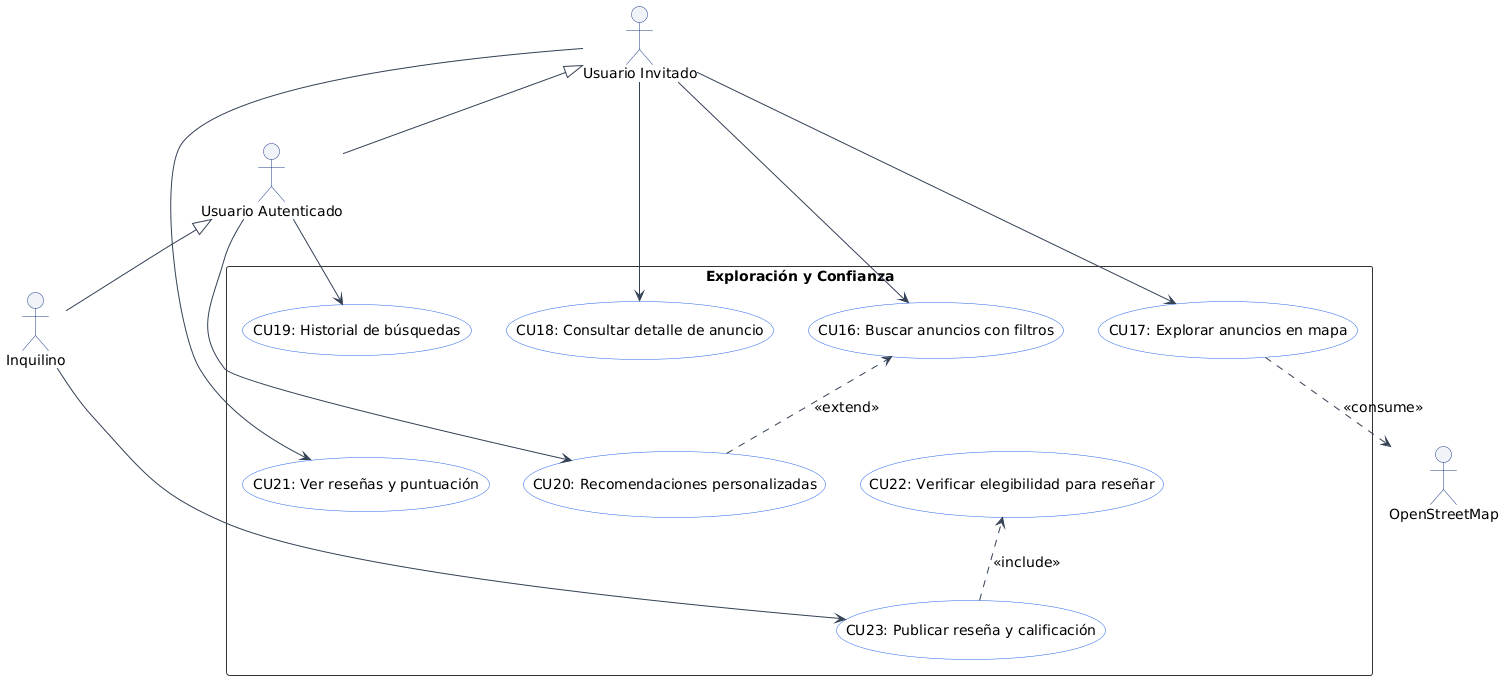
\includegraphics[width=0.88\textwidth]{AnalisisFuncional/img/dcu_busqueda_resenas.png}
    \caption{Diagrama de casos de uso de exploración, recomendaciones y reseñas}
    \label{fig:dcu_busqueda_resenas}
\end{figure}

    Las fichas de especificación funcional para este bloque comprenden desde CU16 hasta CU23:

\begin{table}[H]
\centering
\begin{tabular}{|p{3.1cm}|p{10.9cm}|}
\hline
\textbf{Caso de Uso} & \textbf{CU16: Buscar anuncios con filtros combinados} \\ \hline
\textbf{Actores} & Usuario Invitado, Usuario Autenticado \\ \hline
\textbf{Descripción} & Permite filtrar el catálogo de alojamientos según ciudad, rango de precio, tipo de habitación y servicios incluidos \\ \hline
\textbf{Precondiciones} & Que existan anuncios publicados y activos en la plataforma \\ \hline
\textbf{Flujo básico} & 
1. El usuario accede al explorador del catálogo e introduce los criterios de búsqueda. \newline
2. El sistema consulta la base de datos aplicando los filtros de forma acumulativa. \newline
3. El sistema devuelve los resultados paginados y actualiza la lista visual. \\ \hline
\end{tabular}
\caption{Especificación del caso de uso CU16.}
\label{tab:cu16}
\end{table}

\begin{table}[H]
\centering
\begin{tabular}{|p{3.1cm}|p{10.9cm}|}
\hline
\textbf{Caso de Uso} & \textbf{CU17: Explorar anuncios en mapa interactivo} \\ \hline
\textbf{Actores} & Usuario Invitado, Usuario Autenticado, OpenStreetMap / Nominatim \\ \hline
\textbf{Descripción} & Muestra los anuncios disponibles mediante marcadores geográficos sobre un mapa interactivo \\ \hline
\textbf{Precondiciones} & Disponer de conectividad con el servicio cartográfico \\ \hline
\textbf{Flujo básico} & 
1. El usuario activa la vista de mapa en el catálogo de alojamientos. \newline
2. El cliente solicita los marcadores comprendidos dentro del área geográfica visible. \newline
3. El sistema renderiza las posiciones y permite interactuar con las tarjetas emergentes. \\ \hline
\end{tabular}
\caption{Especificación del caso de uso CU17.}
\label{tab:cu17}
\end{table}

\begin{table}[H]
\centering
\begin{tabular}{|p{3.1cm}|p{10.9cm}|}
\hline
\textbf{Caso de Uso} & \textbf{CU18: Consultar detalle de anuncio y habitaciones} \\ \hline
\textbf{Actores} & Usuario Invitado, Usuario Autenticado \\ \hline
\textbf{Descripción} & Presenta la ficha completa de un anuncio, su galería gráfica, normas, fianza y habitaciones disponibles \\ \hline
\textbf{Precondiciones} & Que el anuncio seleccionado exista y se encuentre en estado visible \\ \hline
\textbf{Flujo básico} & 
1. El usuario pulsa sobre la tarjeta de un alojamiento desde la lista o el mapa. \newline
2. El sistema recupera los datos del inmueble, equipamiento, perfil del anfitrión y reseñas. \newline
3. La interfaz despliega la información organizada en pestañas de detalle. \\ \hline
\end{tabular}
\caption{Especificación del caso de uso CU18.}
\label{tab:cu18}
\end{table}

\begin{table}[H]
\centering
\begin{tabular}{|p{3.1cm}|p{10.9cm}|}
\hline
\textbf{Caso de Uso} & \textbf{CU19: Consultar historial de búsquedas} \\ \hline
\textbf{Actores} & Usuario Autenticado \\ \hline
\textbf{Descripción} & Muestra los términos, rangos de precios y ubicaciones consultadas recientemente \\ \hline
\textbf{Precondiciones} & Mantener una sesión activa con actividad previa registrada \\ \hline
\textbf{Flujo básico} & 
1. El usuario interactúa con la barra de búsqueda o el panel de filtros. \newline
2. El sistema recupera el registro cronológico de consultas previas del usuario. \newline
3. La interfaz presenta sugerencias directas basadas en las preferencias recientes. \\ \hline
\end{tabular}
\caption{Especificación del caso de uso CU19.}
\label{tab:cu19}
\end{table}

\begin{table}[H]
\centering
\begin{tabular}{|p{3.1cm}|p{10.9cm}|}
\hline
\textbf{Caso de Uso} & \textbf{CU20: Obtener recomendaciones personalizadas} \\ \hline
\textbf{Actores} & Usuario Autenticado \\ \hline
\textbf{Descripción} & Extiende la búsqueda de anuncios calculando sugerencias acordes al perfil y búsquedas previas \\ \hline
\textbf{Precondiciones} & Disponer de un historial de navegación con al menos una consulta registrada \\ \hline
\textbf{Flujo básico} & 
1. El usuario accede a la sección de recomendaciones en la pantalla de inicio. \newline
2. El motor de afinidad analiza las búsquedas guardadas y las características del perfil. \newline
3. El sistema ejecuta una búsqueda extendida y devuelve los alojamientos con mayor coincidencia. \\ \hline
\end{tabular}
\caption{Especificación del caso de uso CU20.}
\label{tab:cu20}
\end{table}

\begin{table}[H]
\centering
\begin{tabular}{|p{3.1cm}|p{10.9cm}|}
\hline
\textbf{Caso de Uso} & \textbf{CU21: Ver reseñas y puntuación media} \\ \hline
\textbf{Actores} & Usuario Invitado, Usuario Autenticado \\ \hline
\textbf{Descripción} & Consulta las opiniones, comentarios y calificaciones otorgadas a un alojamiento \\ \hline
\textbf{Precondiciones} & Que la publicación cuente con valoraciones registradas \\ \hline
\textbf{Flujo básico} & 
1. El usuario accede a la pestaña de opiniones dentro de la ficha de detalle. \newline
2. El sistema recupera las reseñas aprobadas y desglosa la media por categorías. \newline
3. La interfaz muestra los comentarios ordenados cronológicamente con la firma del autor. \\ \hline
\end{tabular}
\caption{Especificación del caso de uso CU21.}
\label{tab:cu21}
\end{table}

\begin{table}[H]
\centering
\begin{tabular}{|p{3.1cm}|p{10.9cm}|}
\hline
\textbf{Caso de Uso} & \textbf{CU22: Verificar elegibilidad para reseñar} \\ \hline
\textbf{Actores} & Inquilino \\ \hline
\textbf{Descripción} & Comprueba si el inquilino ha completado una estancia formalmente reservada en el inmueble \\ \hline
\textbf{Precondiciones} & Estar autenticado en el sistema \\ \hline
\textbf{Flujo básico} & 
1. El sistema intercepta el intento de emitir una valoración sobre un alojamiento. \newline
2. El backend audita el histórico de reservas confirmadas y finalizadas del usuario. \newline
3. El sistema comprueba que no exista una valoración previa emitida por la misma estancia. \newline
4. Si la comprobación es favorable, se autoriza la apertura del formulario de reseña. \\ \hline
\end{tabular}
\caption{Especificación del caso de uso CU22.}
\label{tab:cu22}
\end{table}

\begin{table}[H]
\centering
\begin{tabular}{|p{3.1cm}|p{10.9cm}|}
\hline
\textbf{Caso de Uso} & \textbf{CU23: Publicar reseña y calificación} \\ \hline
\textbf{Actores} & Inquilino \\ \hline
\textbf{Descripción} & Registra una valoración numérica de uno a cinco y un comentario descriptivo sobre la estancia \\ \hline
\textbf{Precondiciones} & Haber superado la verificación de elegibilidad previa \\ \hline
\textbf{Flujo básico} & 
1. El inquilino completa las puntuaciones desglosadas y redacta su opinión. \newline
2. Se ejecuta de forma obligatoria la verificación de elegibilidad. \newline
3. El sistema persiste la reseña en la base de datos y recalcula la media del alojamiento. \\ \hline
\end{tabular}
\caption{Especificación del caso de uso CU23.}
\label{tab:cu23}
\end{table}

\subsubsection{Gestión de inmuebles y ciclo de publicación del anfitrión}

    El segundo bloque abarca el registro de la vivienda física, su posicionamiento geográfico, la carga de fotos en Cloudinary y el control de publicación de las habitaciones. La figura \ref{fig:dcu_anfitrion_inmuebles} recoge los ocho casos de uso asociados (CU24 a CU31).

\begin{figure}[H]
    \centering
    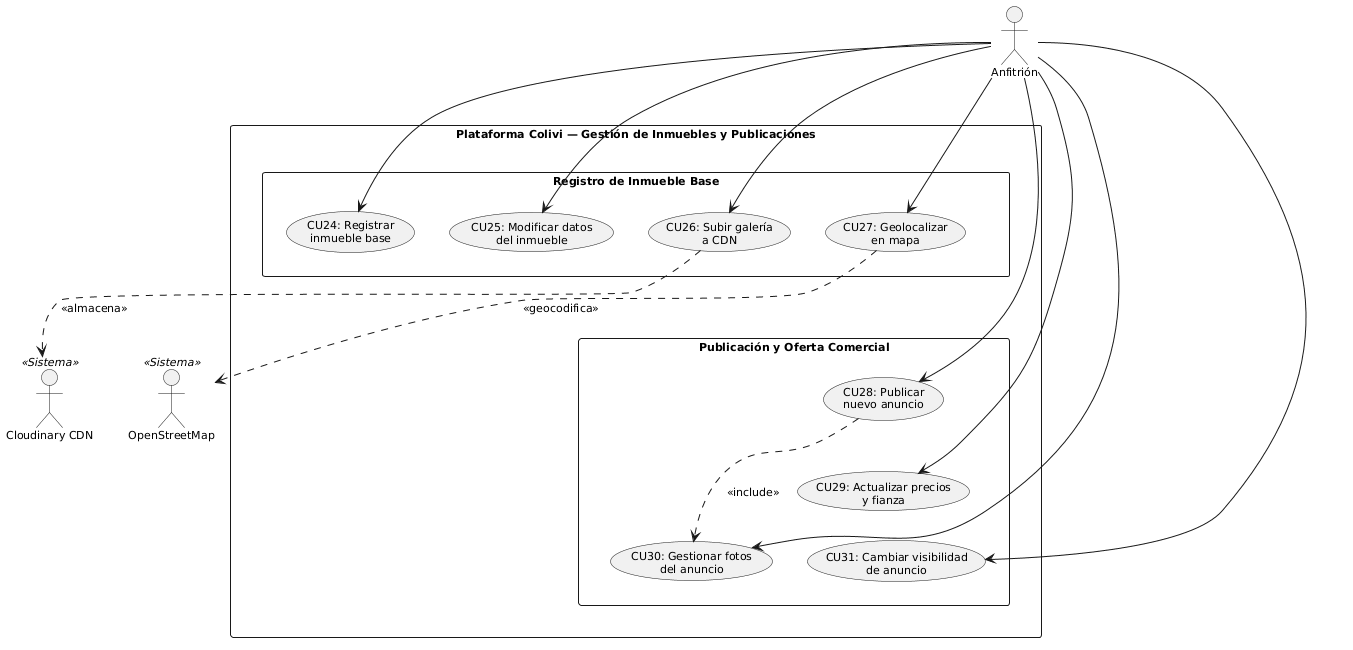
\includegraphics[width=0.88\textwidth]{AnalisisFuncional/img/dcu_anfitrion_inmuebles.png}
    \caption{Diagrama de casos de uso de gestión de inmuebles y publicaciones del anfitrión}
    \label{fig:dcu_anfitrion_inmuebles}
\end{figure}

    Las especificaciones funcionales de este ciclo se detallan desde CU24 hasta CU31:

\begin{table}[H]
\centering
\begin{tabular}{|p{3.1cm}|p{10.9cm}|}
\hline
\textbf{Caso de Uso} & \textbf{CU24: Registrar inmueble base} \\ \hline
\textbf{Actores} & Anfitrión \\ \hline
\textbf{Descripción} & Da de alta la estructura física de una vivienda definiendo superficie, estancias comunes y servicios \\ \hline
\textbf{Precondiciones} & Estar autenticado con perfil de anfitrión \\ \hline
\textbf{Flujo básico} & 
1. El anfitrión accede al asistente de registro de propiedades. \newline
2. El anfitrión especifica la dirección, metros cuadrados, número de habitaciones y zonas comunes. \newline
3. El sistema valida la integridad de los datos y almacena el registro del inmueble base. \\ \hline
\end{tabular}
\caption{Especificación del caso de uso CU24.}
\label{tab:cu24}
\end{table}

\begin{table}[H]
\centering
\begin{tabular}{|p{3.1cm}|p{10.9cm}|}
\hline
\textbf{Caso de Uso} & \textbf{CU25: Modificar datos del inmueble base} \\ \hline
\textbf{Actores} & Anfitrión \\ \hline
\textbf{Descripción} & Permite actualizar la descripción o los equipamientos compartidos de una propiedad \\ \hline
\textbf{Precondiciones} & Ser el titular propietario del inmueble \\ \hline
\textbf{Flujo básico} & 
1. El anfitrión accede al panel de gestión de sus propiedades y selecciona la vivienda. \newline
2. El anfitrión modifica las características físicas o los servicios disponibles. \newline
3. El backend verifica la titularidad y persiste los cambios actualizados. \\ \hline
\end{tabular}
\caption{Especificación del caso de uso CU25.}
\label{tab:cu25}
\end{table}

\begin{table}[H]
\centering
\begin{tabular}{|p{3.1cm}|p{10.9cm}|}
\hline
\textbf{Caso de Uso} & \textbf{CU26: Subir galería fotográfica a CDN} \\ \hline
\textbf{Actores} & Anfitrión, Cloudinary CDN \\ \hline
\textbf{Descripción} & Transfiere un conjunto de imágenes para asociarlas a la ficha del inmueble \\ \hline
\textbf{Precondiciones} & Archivos en formato gráfico admitido que no superen el límite de tamaño establecido \\ \hline
\textbf{Flujo básico} & 
1. El anfitrión selecciona una o varias imágenes desde su explorador local. \newline
2. El cliente transfiere los archivos binarios hacia el servicio de almacenamiento seguro. \newline
3. Cloudinary optimiza y custodia los recursos, retornando los enlaces HTTPS persistentes. \newline
4. El backend almacena las referencias de las imágenes vinculándolas al inmueble. \\ \hline
\end{tabular}
\caption{Especificación del caso de uso CU26.}
\label{tab:cu26}
\end{table}

\begin{table}[H]
\centering
\begin{tabular}{|p{3.1cm}|p{10.9cm}|}
\hline
\textbf{Caso de Uso} & \textbf{CU27: Geolocalizar dirección en mapa} \\ \hline
\textbf{Actores} & Anfitrión, OpenStreetMap / Nominatim \\ \hline
\textbf{Descripción} & Convierte la dirección postal introducida en coordenadas geográficas de latitud y longitud \\ \hline
\textbf{Precondiciones} & Introducir una dirección válida con calle, número, código postal y ciudad \\ \hline
\textbf{Flujo básico} & 
1. El anfitrión escribe la dirección postal durante el alta o edición del inmueble. \newline
2. El cliente remite la consulta al servicio de geocodificación de OpenStreetMap. \newline
3. El servicio devuelve las coordenadas geográficas correspondientes. \newline
4. El sistema posiciona el marcador en el mapa y almacena los valores espaciales. \\ \hline
\end{tabular}
\caption{Especificación del caso de uso CU27.}
\label{tab:cu27}
\end{table}

\begin{table}[H]
\centering
\begin{tabular}{|p{3.1cm}|p{10.9cm}|}
\hline
\textbf{Caso de Uso} & \textbf{CU28: Publicar nuevo anuncio} \\ \hline
\textbf{Actores} & Anfitrión \\ \hline
\textbf{Descripción} & Genera una oferta comercial en el catálogo vinculada a una habitación o al piso completo \\ \hline
\textbf{Precondiciones} & Disponer de un inmueble base registrado con al menos una fotografía \\ \hline
\textbf{Flujo básico} & 
1. El anfitrión pulsa la opción de crear publicación y selecciona el inmueble asociado. \newline
2. El anfitrión fija el título, descripción comercial, renta mensual, fianza y fechas de disponibilidad. \newline
3. Se invoca de forma obligatoria el caso de uso de gestión de fotografías del anuncio. \newline
4. El sistema valida las condiciones económicas y publica la oferta en el catálogo. \\ \hline
\end{tabular}
\caption{Especificación del caso de uso CU28.}
\label{tab:cu28}
\end{table}

\begin{table}[H]
\centering
\begin{tabular}{|p{3.1cm}|p{10.9cm}|}
\hline
\textbf{Caso de Uso} & \textbf{CU29: Actualizar precios, depósito y condiciones} \\ \hline
\textbf{Actores} & Anfitrión \\ \hline
\textbf{Descripción} & Permite reajustar los importes de alquiler, fianza requerida o normas de estancia \\ \hline
\textbf{Precondiciones} & Ser titular del anuncio publicado \\ \hline
\textbf{Flujo básico} & 
1. El anfitrión selecciona el anuncio y abre el formulario de condiciones contractuales. \newline
2. El anfitrión modifica la renta o la fianza y confirma los cambios. \newline
3. El sistema valida que los nuevos importes sean valores numéricos positivos. \newline
4. El backend actualiza la oferta sin alterar las reservas previamente confirmadas. \\ \hline
\end{tabular}
\caption{Especificación del caso de uso CU29.}
\label{tab:cu29}
\end{table}

\begin{table}[H]
\centering
\begin{tabular}{|p{3.1cm}|p{10.9cm}|}
\hline
\textbf{Caso de Uso} & \textbf{CU30: Seleccionar y ordenar imágenes para el anuncio} \\ \hline
\textbf{Actores} & Anfitrión \\ \hline
\textbf{Descripción} & Organiza la galería de fotografías del anuncio y define la imagen de portada principal \\ \hline
\textbf{Precondiciones} & Que el inmueble asociado disponga de imágenes cargadas en el servidor \\ \hline
\textbf{Flujo básico} & 
1. El anfitrión visualiza la cuadrícula de fotografías asignadas a la propiedad. \newline
2. El anfitrión reordena las imágenes y marca la que actuará como cabecera. \newline
3. El sistema guarda la secuencia de ordenamiento para su renderizado en catálogo. \\ \hline
\end{tabular}
\caption{Especificación del caso de uso CU30.}
\label{tab:cu30}
\end{table}

\begin{table}[H]
\centering
\begin{tabular}{|p{3.1cm}|p{10.9cm}|}
\hline
\textbf{Caso de Uso} & \textbf{CU31: Cambiar visibilidad de anuncio} \\ \hline
\textbf{Actores} & Anfitrión \\ \hline
\textbf{Descripción} & Conmuta el estado de una publicación entre disponible, pausada o archivada \\ \hline
\textbf{Precondiciones} & Ser el propietario del anuncio \\ \hline
\textbf{Flujo básico} & 
1. El anfitrión selecciona la acción de cambio de estado en el panel de control. \newline
2. El sistema actualiza el atributo de visibilidad de la publicación. \newline
3. El catálogo omite o incluye el anuncio en los filtros públicos de forma inmediata. \\ \hline
\end{tabular}
\caption{Especificación del caso de uso CU31.}
\label{tab:cu31}
\end{table}
\subsection{Paquete 3: Ciclo de vida de reservas y depósitos}

    El paquete gestiona las propuestas de estancia sobre habitaciones activas, controlando los estados de la reserva y el depósito de garantía económica. Incorpora bloqueos de concurrencia para evitar solapamientos temporales en el calendario cuando múltiples usuarios demandan el mismo periodo. La figura \ref{fig:dcu_reservas} refleja la relación entre actores y los siete casos de uso del módulo (CU32 a CU38).

\begin{figure}[H]
    \centering
    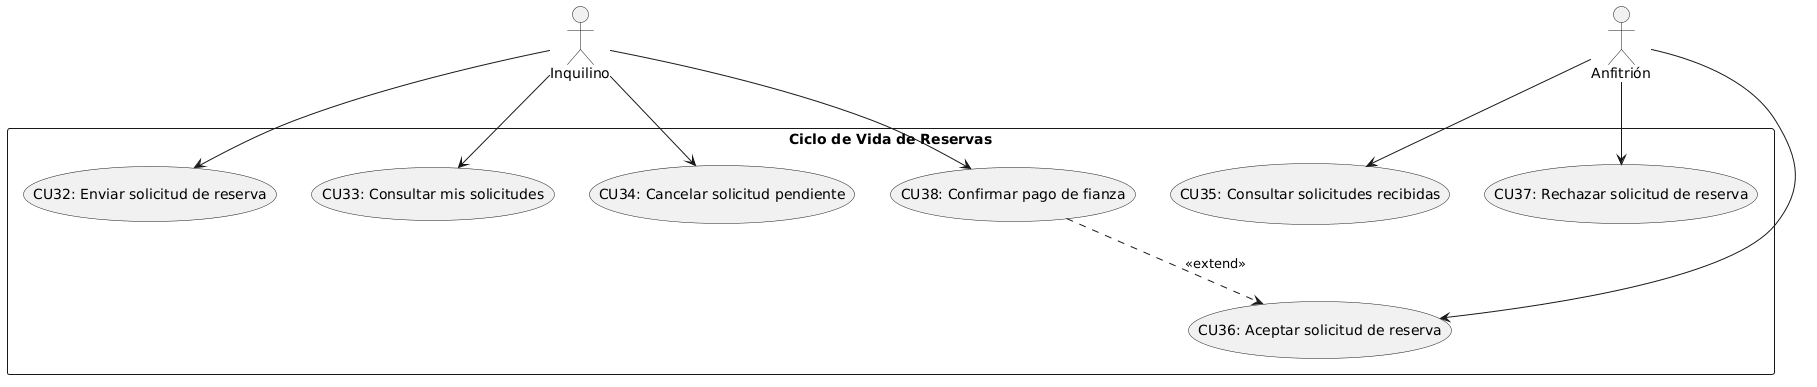
\includegraphics[width=0.75\textwidth]{AnalisisFuncional/img/dcu_reservas.png}
    \caption{Diagrama de casos de uso del ciclo de vida de reservas}
    \label{fig:dcu_reservas}
\end{figure}

    Las fichas descriptivas del ciclo de reserva comprenden desde CU32 hasta CU38:

\begin{table}[H]
\centering
\begin{tabular}{|p{3.2cm}|p{11.3cm}|}
\hline
\textbf{Caso de Uso} & \textbf{CU32: Enviar solicitud de reserva con rango de fechas} \\ \hline
\textbf{Actores} & Inquilino \\ \hline
\textbf{Descripción} & Remite una propuesta de estancia vinculada a un anuncio seleccionando fecha de entrada y salida \\ \hline
\textbf{Precondiciones} & Estar autenticado en la plataforma y no ser el titular del alojamiento \\ \hline
\textbf{Flujo básico} & 
1. El inquilino selecciona las fechas deseadas desde el calendario del anuncio. \newline
2. El sistema comprueba que no existan reservas confirmadas en conflicto temporal. \newline
3. El inquilino redacta un mensaje introductorio y confirma la solicitud. \newline
4. El backend registra la reserva en estado pendiente y notifica al anfitrión. \\ \hline
\end{tabular}
\caption{Especificación del caso de uso CU32.}
\label{tab:cu32}
\end{table}

\begin{table}[H]
\centering
\begin{tabular}{|p{3.2cm}|p{11.3cm}|}
\hline
\textbf{Caso de Uso} & \textbf{CU33: Consultar historial de mis solicitudes} \\ \hline
\textbf{Actores} & Inquilino \\ \hline
\textbf{Descripción} & Muestra el listado de reservas solicitadas por el usuario clasificadas por su estado actual \\ \hline
\textbf{Precondiciones} & Disponer de una sesión activa como inquilino \\ \hline
\textbf{Flujo básico} & 
1. El inquilino accede a su panel de reservas personales. \newline
2. El sistema recupera el registro de solicitudes (pendientes, aceptadas, rechazadas y finalizadas). \newline
3. La interfaz presenta los resúmenes económicos, fechas pactadas y accesos directos. \\ \hline
\end{tabular}
\caption{Especificación del caso de uso CU33.}
\label{tab:cu33}
\end{table}

\begin{table}[H]
\centering
\begin{tabular}{|p{3.2cm}|p{11.3cm}|}
\hline
\textbf{Caso de Uso} & \textbf{CU34: Cancelar solicitud de reserva pendiente} \\ \hline
\textbf{Actores} & Inquilino \\ \hline
\textbf{Descripción} & Permite al inquilino revocar una propuesta antes del pronunciamiento del anfitrión \\ \hline
\textbf{Precondiciones} & Que la reserva se encuentre formalmente en estado pendiente de aprobación \\ \hline
\textbf{Flujo básico} & 
1. El inquilino selecciona la solicitud pendiente y confirma la revocación. \newline
2. El sistema conmuta el estado de la reserva a cancelada. \newline
3. El backend libera el bloqueo preventivo del calendario y remite aviso al propietario. \\ \hline
\end{tabular}
\caption{Especificación del caso de uso CU34.}
\label{tab:cu34}
\end{table}

\begin{table}[H]
\centering
\begin{tabular}{|p{3.2cm}|p{11.3cm}|}
\hline
\textbf{Caso de Uso} & \textbf{CU35: Consultar solicitudes recibidas} \\ \hline
\textbf{Actores} & Anfitrión \\ \hline
\textbf{Descripción} & Despliega las peticiones de estancia pendientes de resolución para los alojamientos del propietario \\ \hline
\textbf{Precondiciones} & Ser titular de al menos un anuncio publicado \\ \hline
\textbf{Flujo básico} & 
1. El anfitrión accede a la bandeja de gestión de solicitudes entrantes. \newline
2. El sistema recupera las peticiones pendientes con el perfil del demandante y su historial. \newline
3. La interfaz expone los detalles temporales y económicos para facilitar la toma de decisión. \\ \hline
\end{tabular}
\caption{Especificación del caso de uso CU35.}
\label{tab:cu35}
\end{table}

\begin{table}[H]
\centering
\begin{tabular}{|p{3.2cm}|p{11.3cm}|}
\hline
\textbf{Caso de Uso} & \textbf{CU36: Aceptar solicitud de reserva} \\ \hline
\textbf{Actores} & Anfitrión \\ \hline
\textbf{Descripción} & Admite formalmente la estancia de un inquilino para el rango de fechas pactado \\ \hline
\textbf{Precondiciones} & Que la solicitud se encuentre en estado pendiente y el calendario disponible \\ \hline
\textbf{Flujo básico} & 
1. El anfitrión examina la petición y pulsa sobre la opción de confirmación. \newline
2. El backend bloquea de forma definitiva las fechas en el calendario del inmueble. \newline
3. El sistema actualiza el estado a aceptada y remite notificación al inquilino. \\ \hline
\end{tabular}
\caption{Especificación del caso de uso CU36.}
\label{tab:cu36}
\end{table}

\begin{table}[H]
\centering
\begin{tabular}{|p{3.2cm}|p{11.3cm}|}
\hline
\textbf{Caso de Uso} & \textbf{CU37: Rechazar solicitud de reserva} \\ \hline
\textbf{Actores} & Anfitrión \\ \hline
\textbf{Descripción} & Deniega una propuesta de estancia detallando de forma opcional el motivo de desestimación \\ \hline
\textbf{Precondiciones} & Que la reserva figure en estado pendiente \\ \hline
\textbf{Flujo básico} & 
1. El anfitrión selecciona la acción de desestimación en la solicitud correspondiente. \newline
2. El anfitrión introduce el motivo de desestimación si lo estima oportuno. \newline
3. El sistema marca la reserva en estado rechazada y actualiza el panel del inquilino. \\ \hline
\end{tabular}
\caption{Especificación del caso de uso CU37.}
\label{tab:cu37}
\end{table}

\begin{table}[H]
\centering
\begin{tabular}{|p{3.2cm}|p{11.3cm}|}
\hline
\textbf{Caso de Uso} & \textbf{CU38: Confirmar y registrar pago de fianza} \\ \hline
\textbf{Actores} & Inquilino \\ \hline
\textbf{Descripción} & Registra el abono del depósito de garantía exigido por el anfitrión para consolidar el contrato \\ \hline
\textbf{Precondiciones} & Que la solicitud de reserva haya sido aceptada previamente por el anfitrión \\ \hline
\textbf{Flujo básico} & 
1. El inquilino accede a su reserva aceptada y pulsa la opción de pago de fianza. \newline
2. El sistema presenta el desglose del importe del depósito establecido. \newline
3. El inquilino introduce los datos de transacción y formaliza la operación. \newline
4. El backend convalida la operación, emite comprobante y consolida la reserva como afianzada. \\ \hline
\end{tabular}
\caption{Especificación del caso de uso CU38.}
\label{tab:cu38}
\end{table}
\subsection{Paquete 4: Comunidad de convivencia y espacio del hogar}

    El paquete estructura la convivencia tras confirmarse el arrendamiento. Permite unir nuevos compañeros mediante códigos dinámicos de un solo uso, personalizar avatares, registrar eventos en un muro de actividad inmutable y tramitar expulsiones o bajas voluntarias siempre que no existan deudas abiertas. La figura \ref{fig:dcu_convivencia} modela los once casos de uso que componen este espacio compartido (CU39 a CU49).

\begin{figure}[H]
    \centering
    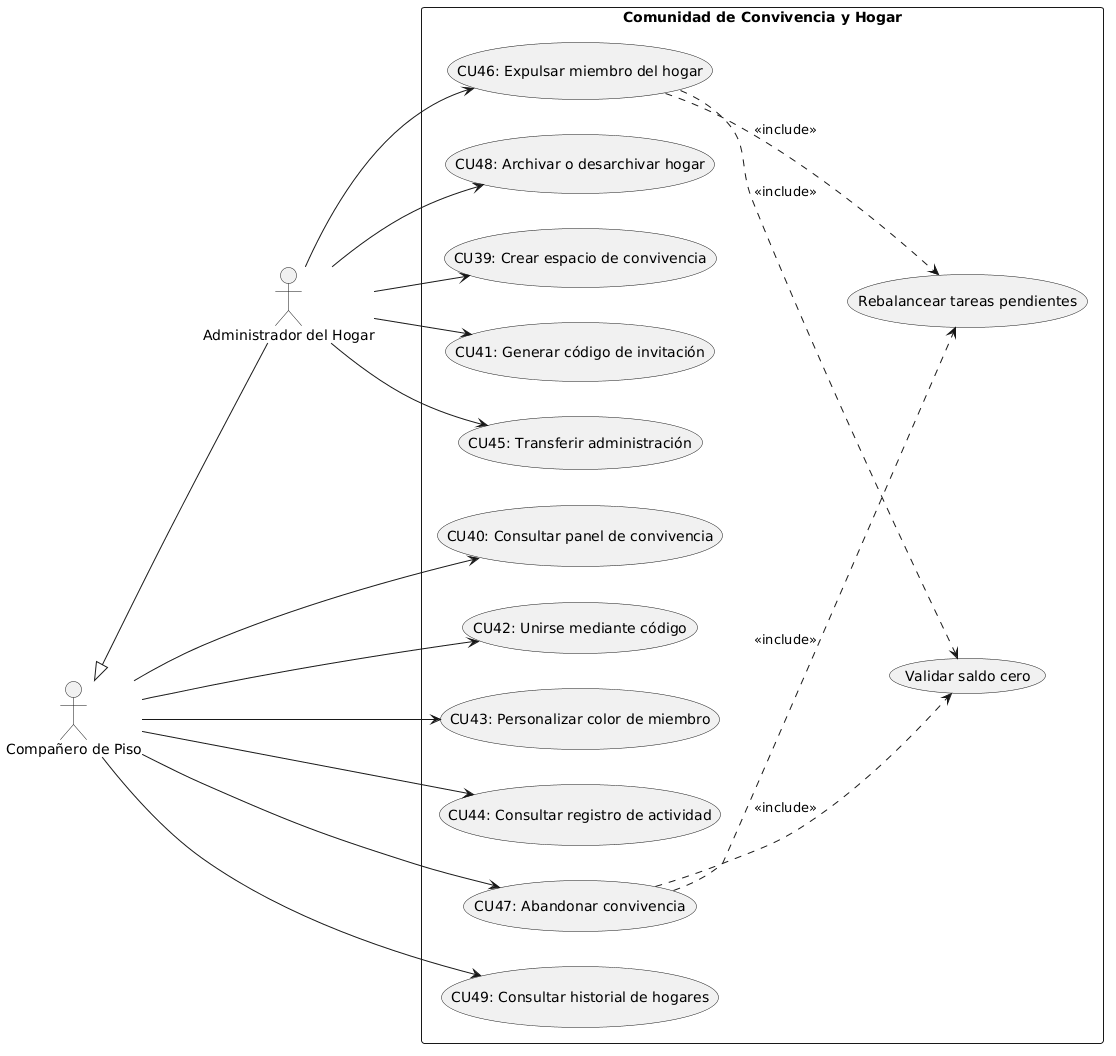
\includegraphics[width=0.85\textwidth]{AnalisisFuncional/img/dcu_convivencia.png}
    \caption{Diagrama de casos de uso de comunidad de convivencia y hogar}
    \label{fig:dcu_convivencia}
\end{figure}

    Las siguientes especificaciones describen los casos de uso asociados al hogar (CU39 a CU49):

\begin{table}[H]
\centering
\begin{tabular}{|p{3.2cm}|p{11.3cm}|}
\hline
\textbf{Caso de Uso} & \textbf{CU39: Crear espacio de convivencia} \\ \hline
\textbf{Actores} & Administrador del Hogar \\ \hline
\textbf{Descripción} & Da de alta un nuevo grupo de piso asignando nombre, dirección y reglas básicas \\ \hline
\textbf{Precondiciones} & Estar autenticado y no pertenecer a otro hogar en calidad de administrador simultáneo \\ \hline
\textbf{Flujo básico} & 
1. El usuario accede al formulario de creación de comunidad e introduce los datos del piso. \newline
2. El sistema valida la información e inicializa el espacio de convivencia. \newline
3. El backend otorga al creador el rol de administrador del hogar. \newline
4. El sistema redirige al panel principal del nuevo hogar. \\ \hline
\end{tabular}
\caption{Especificación del caso de uso CU39}
\label{tab:cu39}
\end{table}

\begin{table}[H]
\centering
\begin{tabular}{|p{3.2cm}|p{11.3cm}|}
\hline
\textbf{Caso de Uso} & \textbf{CU40: Consultar panel y detalle de convivencia} \\ \hline
\textbf{Actores} & Compañero de Piso \\ \hline
\textbf{Descripción} & Muestra la vista global del piso con la lista de miembros, balances rápidos y avisos \\ \hline
\textbf{Precondiciones} & Pertenecer activamente al hogar consultado \\ \hline
\textbf{Flujo básico} & 
1. El usuario accede a la sección de inicio del piso en la interfaz. \newline
2. El sistema recupera los datos de los integrantes, sus roles y estados asignados. \newline
3. La interfaz renderiza el resumen consolidado de convivencia y accesos a módulos. \\ \hline
\end{tabular}
\caption{Especificación del caso de uso CU40}
\label{tab:cu40}
\end{table}

\begin{table}[H]
\centering
\begin{tabular}{|p{3.2cm}|p{11.3cm}|}
\hline
\textbf{Caso de Uso} & \textbf{CU41: Generar o regenerar código de invitación} \\ \hline
\textbf{Actores} & Administrador del Hogar \\ \hline
\textbf{Descripción} & Crea o renueva una clave alfanumérica única para la incorporación de compañeros \\ \hline
\textbf{Precondiciones} & Poseer el rol de administrador en el hogar activo \\ \hline
\textbf{Flujo básico} & 
1. El administrador accede a la sección de invitaciones del piso. \newline
2. El administrador solicita la emisión o sustitución del código de acceso. \newline
3. El backend genera una cadena alfanumérica unívoca e invalida la anterior. \newline
4. La interfaz presenta la clave lista para ser compartida por canales externos. \\ \hline
\end{tabular}
\caption{Especificación del caso de uso CU41}
\label{tab:cu41}
\end{table}

\begin{table}[H]
\centering
\begin{tabular}{|p{3.2cm}|p{11.3cm}|}
\hline
\textbf{Caso de Uso} & \textbf{CU42: Unirse a un hogar mediante código} \\ \hline
\textbf{Actores} & Compañero de Piso \\ \hline
\textbf{Descripción} & Permite a un usuario vincularse a un piso introduciendo la clave de invitación \\ \hline
\textbf{Precondiciones} & Estar autenticado en el sistema y disponer de un código de invitación válido \\ \hline
\textbf{Flujo básico} & 
1. El usuario introduce el código alfanumérico en la pantalla de bienvenida o unirse. \newline
2. El backend verifica la autenticidad y vigencia de la clave introducida. \newline
3. El sistema añade al usuario como compañero activo del hogar. \newline
4. El sistema notifica la incorporación en el muro general de actividad. \\ \hline
\end{tabular}
\caption{Especificación del caso de uso CU42}
\label{tab:cu42}
\end{table}

\begin{table}[H]
\centering
\begin{tabular}{|p{3.2cm}|p{11.3cm}|}
\hline
\textbf{Caso de Uso} & \textbf{CU43: Personalizar color de identificación} \\ \hline
\textbf{Actores} & Compañero de Piso \\ \hline
\textbf{Descripción} & Configura la tonalidad cromática asignada al usuario para calendarios y balances \\ \hline
\textbf{Precondiciones} & Ser miembro activo del piso \\ \hline
\textbf{Flujo básico} & 
1. El compañero abre el selector de color en la configuración de su tarjeta de miembro. \newline
2. El compañero selecciona una tonalidad disponible en la paleta del hogar. \newline
3. El backend persiste la preferencia cromática asociada a la membresía. \newline
4. La interfaz actualiza los distintivos del usuario en tareas y cuadrantes. \\ \hline
\end{tabular}
\caption{Especificación del caso de uso CU43}
\label{tab:cu43}
\end{table}

\begin{table}[H]
\centering
\begin{tabular}{|p{3.2cm}|p{11.3cm}|}
\hline
\textbf{Caso de Uso} & \textbf{CU44: Consultar registro cronológico de actividad} \\ \hline
\textbf{Actores} & Compañero de Piso \\ \hline
\textbf{Descripción} & Despliega el histórico auditable de sucesos relevantes acontecidos en el hogar \\ \hline
\textbf{Precondiciones} & Pertenecer al hogar correspondiente \\ \hline
\textbf{Flujo básico} & 
1. El compañero accede a la pestaña de actividad reciente del piso. \newline
2. El sistema recupera los registros ordenados cronológicamente de forma descendente. \newline
3. La interfaz visualiza eventos de gastos, liquidaciones, tareas y cambios de miembros. \\ \hline
\end{tabular}
\caption{Especificación del caso de uso CU44}
\label{tab:cu44}
\end{table}

\begin{table}[H]
\centering
\begin{tabular}{|p{3.2cm}|p{11.3cm}|}
\hline
\textbf{Caso de Uso} & \textbf{CU45: Transferir privilegios de administrador} \\ \hline
\textbf{Actores} & Administrador del Hogar \\ \hline
\textbf{Descripción} & Traspasa la condición de administrador del espacio a otro compañero de piso \\ \hline
\textbf{Precondiciones} & Ser el administrador vigente y seleccionar un miembro activo diferente \\ \hline
\textbf{Flujo básico} & 
1. El administrador elige a un compañero y pulsa la opción de cesión de privilegios. \newline
2. El sistema solicita confirmación formal para prevenir transferencias involuntarias. \newline
3. El backend reasigna los roles de membresía en la base de datos de manera atómica. \newline
4. El sistema actualiza los permisos de acceso y emite un evento en el feed del hogar. \\ \hline
\end{tabular}
\caption{Especificación del caso de uso CU45}
\label{tab:cu45}
\end{table}

\begin{table}[H]
\centering
\begin{tabular}{|p{3.2cm}|p{11.3cm}|}
\hline
\textbf{Caso de Uso} & \textbf{CU46: Expulsar miembro del hogar} \\ \hline
\textbf{Actores} & Administrador del Hogar \\ \hline
\textbf{Descripción} & Da de baja forzosa a un integrante del piso tras validar la liquidación de sus saldos \\ \hline
\textbf{Precondiciones} & Que el integrante a expulsar no ostente deudas ni créditos pendientes \\ \hline
\textbf{Flujo básico} & 
1. El administrador selecciona la acción de expulsión sobre el integrante. \newline
2. El sistema verifica obligatoriamente que el saldo neto del integrante sea cero. \newline
3. El sistema ejecuta el rebalanceo automático de las tareas domésticas pendientes. \newline
4. El backend conmuta el estado de la membresía a inactiva y revoca sus accesos al piso. \\ \hline
\end{tabular}
\caption{Especificación del caso de uso CU46}
\label{tab:cu46}
\end{table}

\begin{table}[H]
\centering
\begin{tabular}{|p{3.2cm}|p{11.3cm}|}
\hline
\textbf{Caso de Uso} & \textbf{CU47: Abandonar convivencia} \\ \hline
\textbf{Actores} & Compañero de Piso \\ \hline
\textbf{Descripción} & Tramita la baja voluntaria del usuario del espacio de convivencia \\ \hline
\textbf{Precondiciones} & Mantener un balance financiero equilibrado en cero y no ser el único administrador \\ \hline
\textbf{Flujo básico} & 
1. El compañero selecciona la opción de abandonar el hogar desde los ajustes. \newline
2. El sistema comprueba de forma obligatoria que su balance contable sea exactamente cero. \newline
3. El sistema reasigna de manera automática las tareas domésticas que tenía asignadas. \newline
4. El backend desvincula al usuario y archiva su registro histórico en el hogar. \\ \hline
\end{tabular}
\caption{Especificación del caso de uso CU47}
\label{tab:cu47}
\end{table}

\begin{table}[H]
\centering
\begin{tabular}{|p{3.2cm}|p{11.3cm}|}
\hline
\textbf{Caso de Uso} & \textbf{CU48: Archivar o desarchivar vista de hogar} \\ \hline
\textbf{Actores} & Administrador del Hogar \\ \hline
\textbf{Descripción} & Oculta la visualización activa de un piso concluido sin eliminar sus datos históricos \\ \hline
\textbf{Precondiciones} & Que no existan estancias en curso ni deudas monetarias abiertas \\ \hline
\textbf{Flujo básico} & 
1. El administrador activa la conmutación de archivado en la configuración del piso. \newline
2. El sistema comprueba el cierre satisfactorio de todos los compromisos comunes. \newline
3. El backend traslada el hogar al archivo histórico de los participantes. \\ \hline
\end{tabular}
\caption{Especificación del caso de uso CU48}
\label{tab:cu48}
\end{table}

\begin{table}[H]
\centering
\begin{tabular}{|p{3.2cm}|p{11.3cm}|}
\hline
\textbf{Caso de Uso} & \textbf{CU49: Consultar historial de hogares pasados} \\ \hline
\textbf{Actores} & Administrador del Hogar, Compañero de Piso \\ \hline
\textbf{Descripción} & Permite revisar datos y registros de pisos en los que se participó anteriormente \\ \hline
\textbf{Precondiciones} & Haber formado parte de al menos una convivencia finalizada o archivada \\ \hline
\textbf{Flujo básico} & 
1. El usuario accede a la sección de archivos de convivencia en su panel personal. \newline
2. El sistema recupera los expedientes históricos en modo de solo lectura. \newline
3. La interfaz presenta los resúmenes de estancias, compañeros y balances consolidados. \\ \hline
\end{tabular}
\caption{Especificación del caso de uso CU49}
\label{tab:cu49}
\end{table}
\subsection{Paquete 5: Gestión financiera compartida}

    El paquete resuelve la contabilidad compartida entre compañeros de piso. Registra facturas con repartos proporcionales, simplifica grafos de deuda para minimizar transferencias cruzadas y almacena recibos de liquidación directa. La figura \ref{fig:dcu_gastos} detalla las relaciones con los siete casos de uso financieros (CU50 a CU56).

\begin{figure}[H]
    \centering
    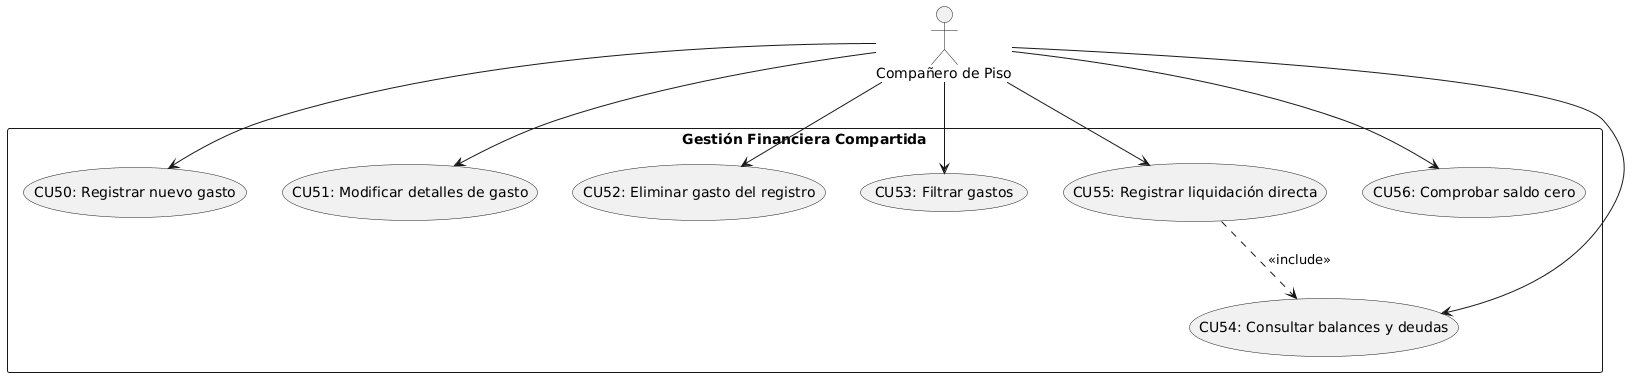
\includegraphics[width=0.75\textwidth]{AnalisisFuncional/img/dcu_gastos.png}
    \caption{Diagrama de casos de uso de gestión financiera compartida}
    \label{fig:dcu_gastos}
\end{figure}

    Las fichas tabulares desglosan los casos de uso CU50 a CU56:

\begin{table}[H]
\centering
\begin{tabular}{|p{3.2cm}|p{11.3cm}|}
\hline
\textbf{Caso de Uso} & \textbf{CU50: Registrar nuevo gasto con reparto} \\ \hline
\textbf{Actores} & Compañero de Piso \\ \hline
\textbf{Descripción} & Introduce un gasto abonado por un miembro distribuyendo el coste entre los integrantes \\ \hline
\textbf{Precondiciones} & Ser miembro activo del hogar con al menos otro compañero vinculado \\ \hline
\textbf{Flujo básico} & 
1. El compañero accede al formulario de gastos e introduce importe, concepto y fecha. \newline
2. El compañero selecciona los participantes asignados al reparto de la cuota. \newline
3. El sistema valida la consistencia matemática entre el total y los importes desglosados. \newline
4. El backend registra la transacción contable y actualiza de inmediato los saldos consolidados. \\ \hline
\end{tabular}
\caption{Especificación del caso de uso CU50}
\label{tab:cu50}
\end{table}

\begin{table}[H]
\centering
\begin{tabular}{|p{3.2cm}|p{11.3cm}|}
\hline
\textbf{Caso de Uso} & \textbf{CU51: Modificar detalles o reparto de gasto} \\ \hline
\textbf{Actores} & Compañero de Piso \\ \hline
\textbf{Descripción} & Permite actualizar la cuantía, concepto o miembros implicados en un gasto registrado \\ \hline
\textbf{Precondiciones} & Ser el creador del registro del gasto y que no pertenezca a un período cerrado \\ \hline
\textbf{Flujo básico} & 
1. El compañero localiza el asiento contable y pulsa sobre la opción de edición. \newline
2. El compañero corrige el importe o reconfigura los miembros que participan. \newline
3. El sistema recalcula las diferencias deudoras y acreedoras asociadas. \newline
4. El backend actualiza la entidad persistida y ajusta los balances generales del hogar. \\ \hline
\end{tabular}
\caption{Especificación del caso de uso CU51}
\label{tab:cu51}
\end{table}

\begin{table}[H]
\centering
\begin{tabular}{|p{3.2cm}|p{11.3cm}|}
\hline
\textbf{Caso de Uso} & \textbf{CU52: Eliminar gasto del registro} \\ \hline
\textbf{Actores} & Compañero de Piso \\ \hline
\textbf{Descripción} & Suprime un gasto registrado previamente revirtiendo su impacto en los balances \\ \hline
\textbf{Precondiciones} & Ostentar la autoría del apunte contable \\ \hline
\textbf{Flujo básico} & 
1. El compañero selecciona el gasto y solicita su retirada formal del historial. \newline
2. El sistema pide confirmación explícita indicando el ajuste contable consecuente. \newline
3. El backend anula la imputación de deuda y restituye los saldos previos de cada miembro. \newline
4. El sistema notifica la supresión del registro en el panel de actividad del piso. \\ \hline
\end{tabular}
\caption{Especificación del caso de uso CU52}
\label{tab:cu52}
\end{table}

\begin{table}[H]
\centering
\begin{tabular}{|p{3.2cm}|p{11.3cm}|}
\hline
\textbf{Caso de Uso} & \textbf{CU53: Filtrar gastos por fechas y participantes} \\ \hline
\textbf{Actores} & Compañero de Piso \\ \hline
\textbf{Descripción} & Permite segmentar el histórico de gastos según intervalos de tiempo o miembros \\ \hline
\textbf{Precondiciones} & Pertenecer al espacio de convivencia consultado \\ \hline
\textbf{Flujo básico} & 
1. El usuario accede a la pestaña de histórico contable en el panel de gastos. \newline
2. El usuario define un rango de fechas, un pagador concreto o un estado de liquidación. \newline
3. El sistema consulta las transacciones coincidentes y devuelve la lista paginada. \newline
4. La interfaz recalcula y muestra la suma total de las operaciones filtradas. \\ \hline
\end{tabular}
\caption{Especificación del caso de uso CU53}
\label{tab:cu53}
\end{table}

\begin{table}[H]
\centering
\begin{tabular}{|p{3.2cm}|p{11.3cm}|}
\hline
\textbf{Caso de Uso} & \textbf{CU54: Consultar balances y transferencias sugeridas} \\ \hline
\textbf{Actores} & Compañero de Piso \\ \hline
\textbf{Descripción} & Muestra el estado neto de saldos y la propuesta óptima de pagos para saldar deudas \\ \hline
\textbf{Precondiciones} & Estar formalmente integrado en el hogar \\ \hline
\textbf{Flujo básico} & 
1. El compañero entra en la vista de balances compartidos. \newline
2. El sistema procesa la matriz de deudas aplicando el algoritmo de simplificación de transferencias. \newline
3. La interfaz visualiza a quién debe dinero cada miembro o cuánto debe percibir. \newline
4. El sistema expone las transacciones sugeridas con importes mínimos para saldar cuentas. \\ \hline
\end{tabular}
\caption{Especificación del caso de uso CU54}
\label{tab:cu54}
\end{table}

\begin{table}[H]
\centering
\begin{tabular}{|p{3.2cm}|p{11.3cm}|}
\hline
\textbf{Caso de Uso} & \textbf{CU55: Registrar liquidación directa} \\ \hline
\textbf{Actores} & Compañero de Piso \\ \hline
\textbf{Descripción} & Asienta un pago directo efectuado entre dos compañeros para compensar una deuda \\ \hline
\textbf{Precondiciones} & Mantener un saldo deudor pendiente respecto al destinatario de la compensación \\ \hline
\textbf{Flujo básico} & 
1. El deudor accede a la lista de transferencias sugeridas y pulsa liquidar saldo. \newline
2. Se invoca de forma obligatoria la consulta de balances y transferencias sugeridas. \newline
3. El usuario confirma el importe transferido y el método de pago utilizado. \newline
4. El backend asienta la liquidación y actualiza los saldos de ambos compañeros a cero. \\ \hline
\end{tabular}
\caption{Especificación del caso de uso CU55}
\label{tab:cu55}
\end{table}

\begin{table}[H]
\centering
\begin{tabular}{|p{3.2cm}|p{11.3cm}|}
\hline
\textbf{Caso de Uso} & \textbf{CU56: Comprobar saldo cero} \\ \hline
\textbf{Actores} & Compañero de Piso \\ \hline
\textbf{Descripción} & Valida automáticamente que un miembro no posea deudas activas ni acreencias en el piso \\ \hline
\textbf{Precondiciones} & Estar en proceso de abandono o expulsión del espacio de convivencia \\ \hline
\textbf{Flujo básico} & 
1. El sistema intercepta una solicitud de baja voluntaria o expulsión de un miembro. \newline
2. El backend computa el balance neto acumulado del usuario en todos los gastos registrados. \newline
3. Si el saldo es exactamente cero, el sistema confirma la validación favorablemente. \newline
4. Si existe balance positivo o negativo, el sistema bloquea la operación e indica la liquidación previa. \\ \hline
\end{tabular}
\caption{Especificación del caso de uso CU56}
\label{tab:cu56}
\end{table}
\subsection{Paquete 6: Motor de tareas domésticas y sistema de puntos}

    El paquete automatiza la asignación y supervisión de las tareas del hogar. Implementa un motor de rotación equitativa (\emph{Round-Robin}), un calendario compartido de turnos, incentivos gamificados mediante puntuaciones y una función de rescate para tareas vencidas. La figura \ref{fig:dcu_tareas} expone los siete casos de uso del subsistema (CU57 a CU63).

\begin{figure}[H]
    \centering
    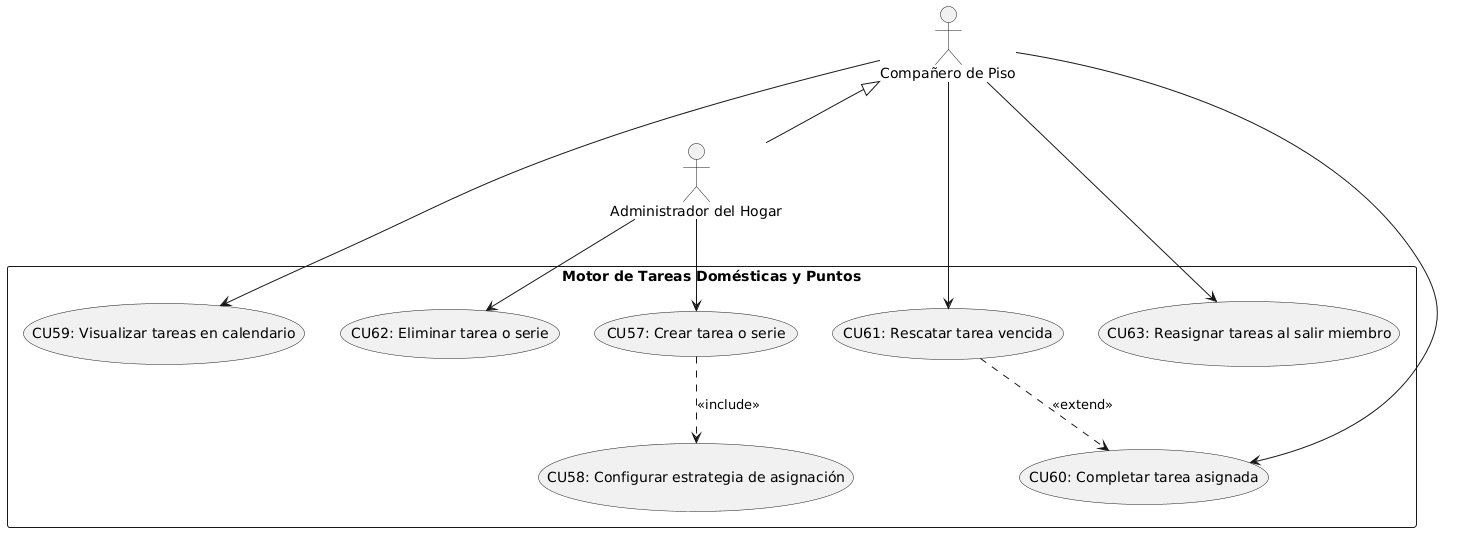
\includegraphics[width=0.78\textwidth]{AnalisisFuncional/img/dcu_tareas.png}
    \caption{Diagrama de casos de uso de tareas domésticas y puntos}
    \label{fig:dcu_tareas}
\end{figure}

    Las siguientes fichas estructuran el comportamiento de CU57 a CU63:

\begin{table}[H]
\centering
\begin{tabular}{|p{3.2cm}|p{11.3cm}|}
\hline
\textbf{Caso de Uso} & \textbf{CU57: Crear tarea única o serie recurrente} \\ \hline
\textbf{Actores} & Administrador del Hogar \\ \hline
\textbf{Descripción} & Da de alta una labor doméstica puntual o una serie periódica vinculada a un valor en puntos \\ \hline
\textbf{Precondiciones} & Ostentar el rol de administrador en el hogar correspondiente \\ \hline
\textbf{Flujo básico} & 
1. El administrador accede al planificador de tareas y pulsa sobre la opción de nueva labor. \newline
2. El administrador define el título, descripción, periodicidad, fecha límite y recompensa en puntos. \newline
3. Se invoca de forma obligatoria la configuración de la estrategia de asignación de miembros. \newline
4. El backend genera la serie o tarea única y la incorpora al calendario general del piso. \\ \hline
\end{tabular}
\caption{Especificación del caso de uso CU57}
\label{tab:cu57}
\end{table}

\begin{table}[H]
\centering
\begin{tabular}{|p{3.2cm}|p{11.3cm}|}
\hline
\textbf{Caso de Uso} & \textbf{CU58: Configurar estrategia de asignación} \\ \hline
\textbf{Actores} & Administrador del Hogar \\ \hline
\textbf{Descripción} & Determina la política de adjudicación de turnos entre fija o rotativa equitativa \\ \hline
\textbf{Precondiciones} & Estar en proceso de creación o parametrización de una labor doméstica \\ \hline
\textbf{Flujo básico} & 
1. El administrador elige si la tarea recae siempre en un miembro fijo o en una secuencia cíclica. \newline
2. En caso rotativo, el sistema ordena a los compañeros activos para repartir la carga. \newline
3. El motor de planificación almacena el orden de turnos asociado a la serie. \\ \hline
\end{tabular}
\caption{Especificación del caso de uso CU58}
\label{tab:cu58}
\end{table}

\begin{table}[H]
\centering
\begin{tabular}{|p{3.2cm}|p{11.3cm}|}
\hline
\textbf{Caso de Uso} & \textbf{CU59: Visualizar tareas en calendario y cuadrante} \\ \hline
\textbf{Actores} & Compañero de Piso \\ \hline
\textbf{Descripción} & Muestra el estado de las labores domésticas en formato de cuadrante mensual o lista diaria \\ \hline
\textbf{Precondiciones} & Formar parte activa del espacio de convivencia \\ \hline
\textbf{Flujo básico} & 
1. El compañero abre el panel de tareas domésticas en la interfaz. \newline
2. El sistema recupera las tareas programadas con su estado (pendiente, completada o vencida). \newline
3. La interfaz renderiza las labores diferenciando a los asignatarios por su código de color. \\ \hline
\end{tabular}
\caption{Especificación del caso de uso CU59}
\label{tab:cu59}
\end{table}

\begin{table}[H]
\centering
\begin{tabular}{|p{3.2cm}|p{11.3cm}|}
\hline
\textbf{Caso de Uso} & \textbf{CU60: Completar tarea asignada} \\ \hline
\textbf{Actores} & Compañero de Piso \\ \hline
\textbf{Descripción} & Marca una labor asignada como finalizada sumando los puntos previstos al perfil \\ \hline
\textbf{Precondiciones} & Que la tarea figure asignada al usuario y no se encuentre ya convalidada \\ \hline
\textbf{Flujo básico} & 
1. El compañero selecciona su tarea pendiente en el cuadrante y confirma su realización. \newline
2. El backend marca la labor en estado completada y registra la marca de tiempo de cierre. \newline
3. El sistema añade los puntos de recompensa al balance de gamificación del usuario. \newline
4. Si la tarea formaba parte de una serie rotativa, el sistema planifica la siguiente iteración. \\ \hline
\end{tabular}
\caption{Especificación del caso de uso CU60}
\label{tab:cu60}
\end{table}

\begin{table}[H]
\centering
\begin{tabular}{|p{3.2cm}|p{11.3cm}|}
\hline
\textbf{Caso de Uso} & \textbf{CU61: Rescatar tarea vencida de otro miembro} \\ \hline
\textbf{Actores} & Compañero de Piso \\ \hline
\textbf{Descripción} & Asume y completa una labor fuera de plazo no realizada por otro compañero sumando puntos extra \\ \hline
\textbf{Precondiciones} & Que la labor se encuentre formalmente vencida y asignada originalmente a otro compañero \\ \hline
\textbf{Flujo básico} & 
1. El compañero localiza una tarea expirada en el tablón común y activa la opción de rescate. \newline
2. El sistema transfiere de forma transitoria la asignación de la labor al nuevo usuario. \newline
3. Se invoca de forma extendida el caso de uso de completar tarea asignada. \newline
4. El sistema asigna la bonificación de puntos al rescatador y emite notificación al piso. \\ \hline
\end{tabular}
\caption{Especificación del caso de uso CU61}
\label{tab:cu61}
\end{table}

\begin{table}[H]
\centering
\begin{tabular}{|p{3.2cm}|p{11.3cm}|}
\hline
\textbf{Caso de Uso} & \textbf{CU62: Eliminar tarea o serie recurrente} \\ \hline
\textbf{Actores} & Administrador del Hogar \\ \hline
\textbf{Descripción} & Da de baja una tarea programada o cancela de manera definitiva una serie recurrente \\ \hline
\textbf{Precondiciones} & Poseer privilegios de administración en el espacio doméstico \\ \hline
\textbf{Flujo básico} & 
1. El administrador selecciona la labor a suprimir y elige entre borrar la instancia o la serie entera. \newline
2. El sistema solicita confirmación advirtiendo sobre las asignaciones futuras afectadas. \newline
3. El backend purga los registros planificados y recalcula el calendario del hogar. \\ \hline
\end{tabular}
\caption{Especificación del caso de uso CU62}
\label{tab:cu62}
\end{table}

\begin{table}[H]
\centering
\begin{tabular}{|p{3.2cm}|p{11.3cm}|}
\hline
\textbf{Caso de Uso} & \textbf{CU63: Reasignar tareas al salir un miembro} \\ \hline
\textbf{Actores} & Compañero de Piso, Administrador del Hogar \\ \hline
\textbf{Descripción} & Redistribuye automáticamente las labores que estaban asignadas a un miembro saliente \\ \hline
\textbf{Precondiciones} & Que un miembro abandone el piso o sea expulsado formalmente \\ \hline
\textbf{Flujo básico} & 
1. El sistema intercepta el proceso de desvinculación formal de un integrante. \newline
2. El backend audita todas las tareas pendientes o futuras asociadas al usuario saliente. \newline
3. El motor de rotación redistribuye las responsabilidades entre los miembros restantes. \newline
4. El sistema notifica la actualización del cuadrante a los compañeros activos. \\ \hline
\end{tabular}
\caption{Especificación del caso de uso CU63}
\label{tab:cu63}
\end{table}
\subsection{Paquete 7: Mensajería contextual}

    El canal de mensajería vincula cada hilo de chat con el anuncio correspondiente. Permite que inquilinos y propietarios intercambien mensajes antes o después de reservar, manteniendo el histórico de comunicaciones, el estado de lectura y la trazabilidad necesaria ante disputas. La figura \ref{fig:dcu_mensajeria} esquematiza los cinco casos de uso del módulo (CU64 a CU68).

\begin{figure}[H]
    \centering
    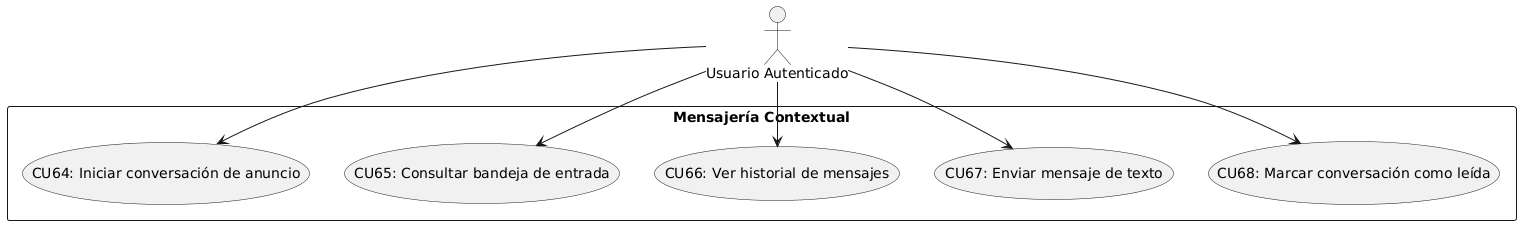
\includegraphics[width=0.75\textwidth]{AnalisisFuncional/img/dcu_mensajeria.png}
    \caption{Diagrama de casos de uso de mensajería contextual}
    \label{fig:dcu_mensajeria}
\end{figure}

    Las siguientes tablas recogen la especificación de CU64 a CU68:

\begin{table}[H]
\centering
\begin{tabular}{|p{3.2cm}|p{11.3cm}|}
\hline
\textbf{Caso de Uso} & \textbf{CU64: Iniciar conversación vinculada a un anuncio} \\ \hline
\textbf{Actores} & Usuario Autenticado \\ \hline
\textbf{Descripción} & Abre un nuevo hilo de chat directo entre el usuario y el anfitrión de una publicación \\ \hline
\textbf{Precondiciones} & Estar autenticado, que el anuncio esté activo y no ser el propio propietario del mismo \\ \hline
\textbf{Flujo básico} & 
1. El usuario accede a la ficha de un alojamiento y pulsa sobre la opción de contactar. \newline
2. El sistema comprueba si ya existía una conversación previa abierta para ese contexto. \newline
3. Si existe, redirige al hilo histórico; en caso contrario, inicializa un nuevo canal vinculado. \newline
4. La interfaz abre la ventana de conversación lista para la redacción de mensajes. \\ \hline
\end{tabular}
\caption{Especificación del caso de uso CU64}
\label{tab:cu64}
\end{table}

\begin{table}[H]
\centering
\begin{tabular}{|p{3.2cm}|p{11.3cm}|}
\hline
\textbf{Caso de Uso} & \textbf{CU65: Consultar bandeja de entrada y no leídos} \\ \hline
\textbf{Actores} & Usuario Autenticado \\ \hline
\textbf{Descripción} & Despliega la relación de hilos de mensajería del usuario con indicadores de mensajes pendientes \\ \hline
\textbf{Precondiciones} & Mantener una sesión autenticada activa \\ \hline
\textbf{Flujo básico} & 
1. El usuario accede a la sección de mensajes desde la barra superior de navegación. \newline
2. El sistema recupera las conversaciones activas ordenadas por la fecha del último mensaje. \newline
3. La interfaz presenta los resúmenes de cada chat, los avatares y el recuento de no leídos. \\ \hline
\end{tabular}
\caption{Especificación del caso de uso CU65}
\label{tab:cu65}
\end{table}

\begin{table}[H]
\centering
\begin{tabular}{|p{3.2cm}|p{11.3cm}|}
\hline
\textbf{Caso de Uso} & \textbf{CU66: Ver historial de mensajes} \\ \hline
\textbf{Actores} & Usuario Autenticado \\ \hline
\textbf{Descripción} & Carga y visualiza la secuencia cronológica de intervenciones dentro de una conversación \\ \hline
\textbf{Precondiciones} & Ser participante legítimo (emisor o receptor) de la conversación seleccionada \\ \hline
\textbf{Flujo básico} & 
1. El usuario selecciona un hilo de conversación de su bandeja de entrada. \newline
2. El backend verifica la pertenencia del usuario al hilo solicitado. \newline
3. El sistema devuelve los mensajes paginados con sus marcas de tiempo asociadas. \newline
4. La interfaz renderiza el diálogo diferenciando visualmente los mensajes propios y ajenos. \\ \hline
\end{tabular}
\caption{Especificación del caso de uso CU66}
\label{tab:cu66}
\end{table}

\begin{table}[H]
\centering
\begin{tabular}{|p{3.2cm}|p{11.3cm}|}
\hline
\textbf{Caso de Uso} & \textbf{CU67: Enviar mensaje de texto} \\ \hline
\textbf{Actores} & Usuario Autenticado \\ \hline
\textbf{Descripción} & Transmite un nuevo mensaje de texto plano hacia el destinatario en el hilo activo \\ \hline
\textbf{Precondiciones} & Formar parte de la conversación y que el contenido no supere los límites de longitud \\ \hline
\textbf{Flujo básico} & 
1. El usuario introduce el texto en el área de entrada del chat y pulsa enviar. \newline
2. El cliente valida que el cuerpo del mensaje no se encuentre vacío. \newline
3. El backend persiste el mensaje en base de datos con la marca temporal actual. \newline
4. El sistema notifica al receptor y actualiza la vista de la conversación en tiempo real. \\ \hline
\end{tabular}
\caption{Especificación del caso de uso CU67}
\label{tab:cu67}
\end{table}

\begin{table}[H]
\centering
\begin{tabular}{|p{3.2cm}|p{11.3cm}|}
\hline
\textbf{Caso de Uso} & \textbf{CU68: Marcar conversación como leída} \\ \hline
\textbf{Actores} & Usuario Autenticado \\ \hline
\textbf{Descripción} & Actualiza el estado de los mensajes entrantes poniendo a cero los indicadores pendientes \\ \hline
\textbf{Precondiciones} & Tener mensajes recibidos no leídos en el hilo visualizado \\ \hline
\textbf{Flujo básico} & 
1. El usuario abre o mantiene en foco una conversación con mensajes pendientes. \newline
2. El cliente emite una petición asíncrona informando de la visualización del hilo. \newline
3. El backend actualiza la marca de lectura de los mensajes correspondientes. \newline
4. La interfaz disminuye o suprime los distintivos numéricos de notificación global. \\ \hline
\end{tabular}
\caption{Especificación del caso de uso CU68}
\label{tab:cu68}
\end{table}
\subsection{Paquete 8: Asistente inteligente y orquestación de herramientas}

    El asistente virtual responde consultas en lenguaje natural apoyándose en Spring AI y en un servidor MCP (\emph{Model Context Protocol}). Permite filtrar habitaciones, consultar el estado de las tareas del hogar, resumir la mensajería entrante e inspeccionar colas de moderación. Para proteger los datos, el backend expide tickets efímeros con permisos de solo lectura antes de invocar las herramientas MCP. La figura \ref{fig:dcu_asistente_ia} expone los siete casos de uso del asistente (CU69 a CU75).

\begin{figure}[H]
    \centering
    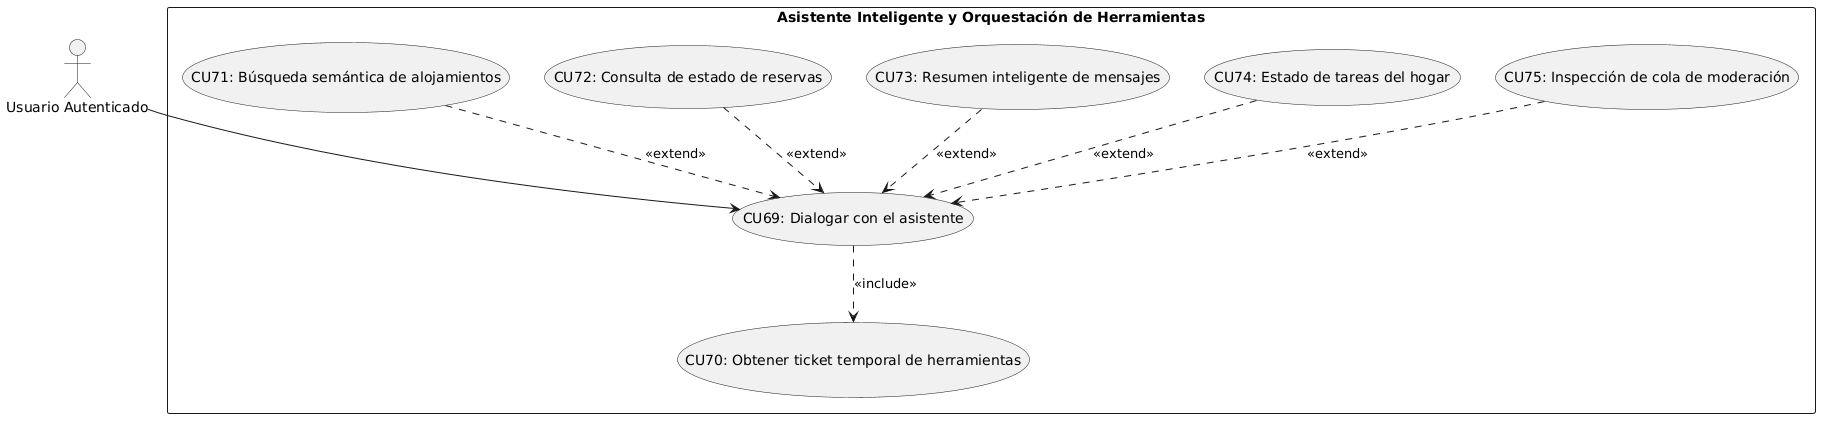
\includegraphics[width=0.82\textwidth]{AnalisisFuncional/img/dcu_asistente_ia.png}
    \caption{Diagrama de casos de uso de asistente inteligente y orquestación de herramientas}
    \label{fig:dcu_asistente_ia}
\end{figure}

    Las siguientes tablas detallan los casos de uso del agente inteligente (CU69 a CU75):

\begin{table}[H]
\centering
\begin{tabular}{|p{3.2cm}|p{11.3cm}|}
\hline
\textbf{Caso de Uso} & \textbf{CU69: Dialogar con el asistente en lenguaje natural} \\ \hline
\textbf{Actores} & Usuario Autenticado \\ \hline
\textbf{Descripción} & Mantiene una conversación interactiva con el agente inteligente mediante lenguaje natural \\ \hline
\textbf{Precondiciones} & Estar autenticado con una sesión activa en la aplicación \\ \hline
\textbf{Flujo básico} & 
1. El usuario abre el componente flotante de chat con el asistente e introduce una consulta. \newline
2. Se ejecuta de forma obligatoria la expedición de un ticket temporal de autorización para herramientas. \newline
3. El orquestador del backend procesa la petición evaluando si requiere invocar herramientas especializadas. \newline
4. El modelo genera la respuesta estructurada y la interfaz la visualiza mediante transmisión progresiva. \\ \hline
\end{tabular}
\caption{Especificación del caso de uso CU69}
\label{tab:cu69}
\end{table}

\begin{table}[H]
\centering
\begin{tabular}{|p{3.2cm}|p{11.3cm}|}
\hline
\textbf{Caso de Uso} & \textbf{CU70: Obtener ticket temporal de autenticación de herramientas} \\ \hline
\textbf{Actores} & Usuario Autenticado \\ \hline
\textbf{Descripción} & Emite una credencial temporal firmada para autorizar llamadas seguras al servidor de herramientas MCP \\ \hline
\textbf{Precondiciones} & Mantener un token de sesión JWT válido \\ \hline
\textbf{Flujo básico} & 
1. El subsistema de inteligencia artificial intercepta la interacción del usuario autenticado. \newline
2. El servicio emite un ticket criptográfico de corta duración vinculado al identificador del usuario. \newline
3. El backend traslada el ticket en las cabeceras de comunicación con el servidor MCP. \newline
4. El servidor MCP convalida la firma del ticket garantizando el aislamiento de privilegios. \\ \hline
\end{tabular}
\caption{Especificación del caso de uso CU70}
\label{tab:cu70}
\end{table}

\begin{table}[H]
\centering
\begin{tabular}{|p{3.2cm}|p{11.3cm}|}
\hline
\textbf{Caso de Uso} & \textbf{CU71: Herramienta: Búsqueda semántica por preferencias} \\ \hline
\textbf{Actores} & Usuario Autenticado \\ \hline
\textbf{Descripción} & Recupera anuncios considerando el estilo de vida, afinidad y descriptores cualitativos del usuario \\ \hline
\textbf{Precondiciones} & Que la consulta del usuario exprese requerimientos de convivencia o preferencias ambientales \\ \hline
\textbf{Flujo básico} & 
1. El modelo identifica la intención de localización cualitativa durante el diálogo con el asistente. \newline
2. El agente invoca de forma extendida la herramienta de búsqueda semántica con los criterios extraídos. \newline
3. El servidor MCP consulta el catálogo indexado y devuelve los alojamientos con mayor afinidad contextual. \newline
4. El asistente sintetiza la respuesta recomendando los inmuebles más adecuados en la conversación. \\ \hline
\end{tabular}
\caption{Especificación del caso de uso CU71}
\label{tab:cu71}
\end{table}

\begin{table}[H]
\centering
\begin{tabular}{|p{3.2cm}|p{11.3cm}|}
\hline
\textbf{Caso de Uso} & \textbf{CU72: Herramienta: Consulta de estado de reservas} \\ \hline
\textbf{Actores} & Usuario Autenticado \\ \hline
\textbf{Descripción} & Comprueba y resume el estado actual de las solicitudes de reserva emitidas o recibidas \\ \hline
\textbf{Precondiciones} & Que el usuario pregunte expresamente sobre la situación de sus estancias o reservas \\ \hline
\textbf{Flujo básico} & 
1. El modelo detecta una petición sobre el progreso de las reservas en curso. \newline
2. El agente ejecuta la llamada a la herramienta MCP transmitiendo el contexto de identidad del usuario. \newline
3. El servicio consulta la base de datos y compila las reservas pendientes, aceptadas o próximas a expirar. \newline
4. El asistente traslada un resumen conciso indicando las acciones pendientes que requiere cada solicitud. \\ \hline
\end{tabular}
\caption{Especificación del caso de uso CU72}
\label{tab:cu72}
\end{table}

\begin{table}[H]
\centering
\begin{tabular}{|p{3.2cm}|p{11.3cm}|}
\hline
\textbf{Caso de Uso} & \textbf{CU73: Herramienta: Resumen inteligente de mensajes} \\ \hline
\textbf{Actores} & Usuario Autenticado \\ \hline
\textbf{Descripción} & Sintetiza los temas clave y mensajes no leídos acumulados en la bandeja de entrada \\ \hline
\textbf{Precondiciones} & Disponer de mensajes recibidos en las conversaciones de la plataforma \\ \hline
\textbf{Flujo básico} & 
1. El usuario solicita al asistente conocer las novedades de sus conversaciones activas. \newline
2. El agente ejecuta condicionalmente la herramienta de agregación y análisis de mensajería. \newline
3. El servidor MCP recopila los hilos recientes omitiendo información confidencial no pertinente. \newline
4. El modelo estructura un extracto de las comunicaciones pendientes organizadas por remitente y urgencia. \\ \hline
\end{tabular}
\caption{Especificación del caso de uso CU73}
\label{tab:cu73}
\end{table}

\begin{table}[H]
\centering
\begin{tabular}{|p{3.2cm}|p{11.3cm}|}
\hline
\textbf{Caso de Uso} & \textbf{CU74: Herramienta: Estado de tareas del hogar} \\ \hline
\textbf{Actores} & Usuario Autenticado \\ \hline
\textbf{Descripción} & Proporciona una panorámica rápida sobre las tareas domésticas pendientes y las fechas límite en el piso \\ \hline
\textbf{Precondiciones} & Pertenecer activamente a un hogar constituido \\ \hline
\textbf{Flujo básico} & 
1. El usuario consulta mediante lenguaje natural por las labores domésticas que tiene pendientes. \newline
2. El asistente activa la herramienta MCP correspondiente consultando el módulo del hogar del usuario. \newline
3. El servicio devuelve las tareas asignadas para la semana, turnos rotativos y tareas susceptibles de rescate. \newline
4. El modelo expone el estado de las labores recordando los puntos asignados a cada una. \\ \hline
\end{tabular}
\caption{Especificación del caso de uso CU74}
\label{tab:cu74}
\end{table}

\begin{table}[H]
\centering
\begin{tabular}{|p{3.2cm}|p{11.3cm}|}
\hline
\textbf{Caso de Uso} & \textbf{CU75: Herramienta: Inspección de cola de moderación} \\ \hline
\textbf{Actores} & Usuario Autenticado \\ \hline
\textbf{Descripción} & Asiste en la revisión y diagnóstico rápido de reportes pendientes acumulados en la cola de incidencias \\ \hline
\textbf{Precondiciones} & Poseer el rol de administración del sistema (\emph{ADMIN}) \\ \hline
\textbf{Flujo básico} & 
1. Un administrador del sistema consulta al asistente sobre la carga actual de denuncias sin resolver. \newline
2. El agente comprueba los privilegios de administración del emisor y llama a la herramienta interna MCP. \newline
3. El servicio recopila las infracciones más graves y los usuarios reincidentes en la cola de moderación. \newline
4. El asistente sintetiza los expedientes prioritarios facilitando la toma de decisiones sancionadoras. \\ \hline
\end{tabular}
\caption{Especificación del caso de uso CU75}
\label{tab:cu75}
\end{table}
\subsection{Paquete 9: Panel de administración, gobernanza y moderación global}

    El paquete gestiona las funciones disciplinarias y la mediación en disputas dentro de la plataforma. Cualquier usuario puede denunciar comportamientos contrarios a las normas de convivencia, mientras que los administradores revisan chats notificados, resuelven quejas en bloque y sancionan infractores inhabilitando cuentas o retirando anuncios. La figura \ref{fig:dcu_moderacion} reúne los once casos de uso del módulo (CU76 a CU86).

\begin{figure}[H]
    \centering
    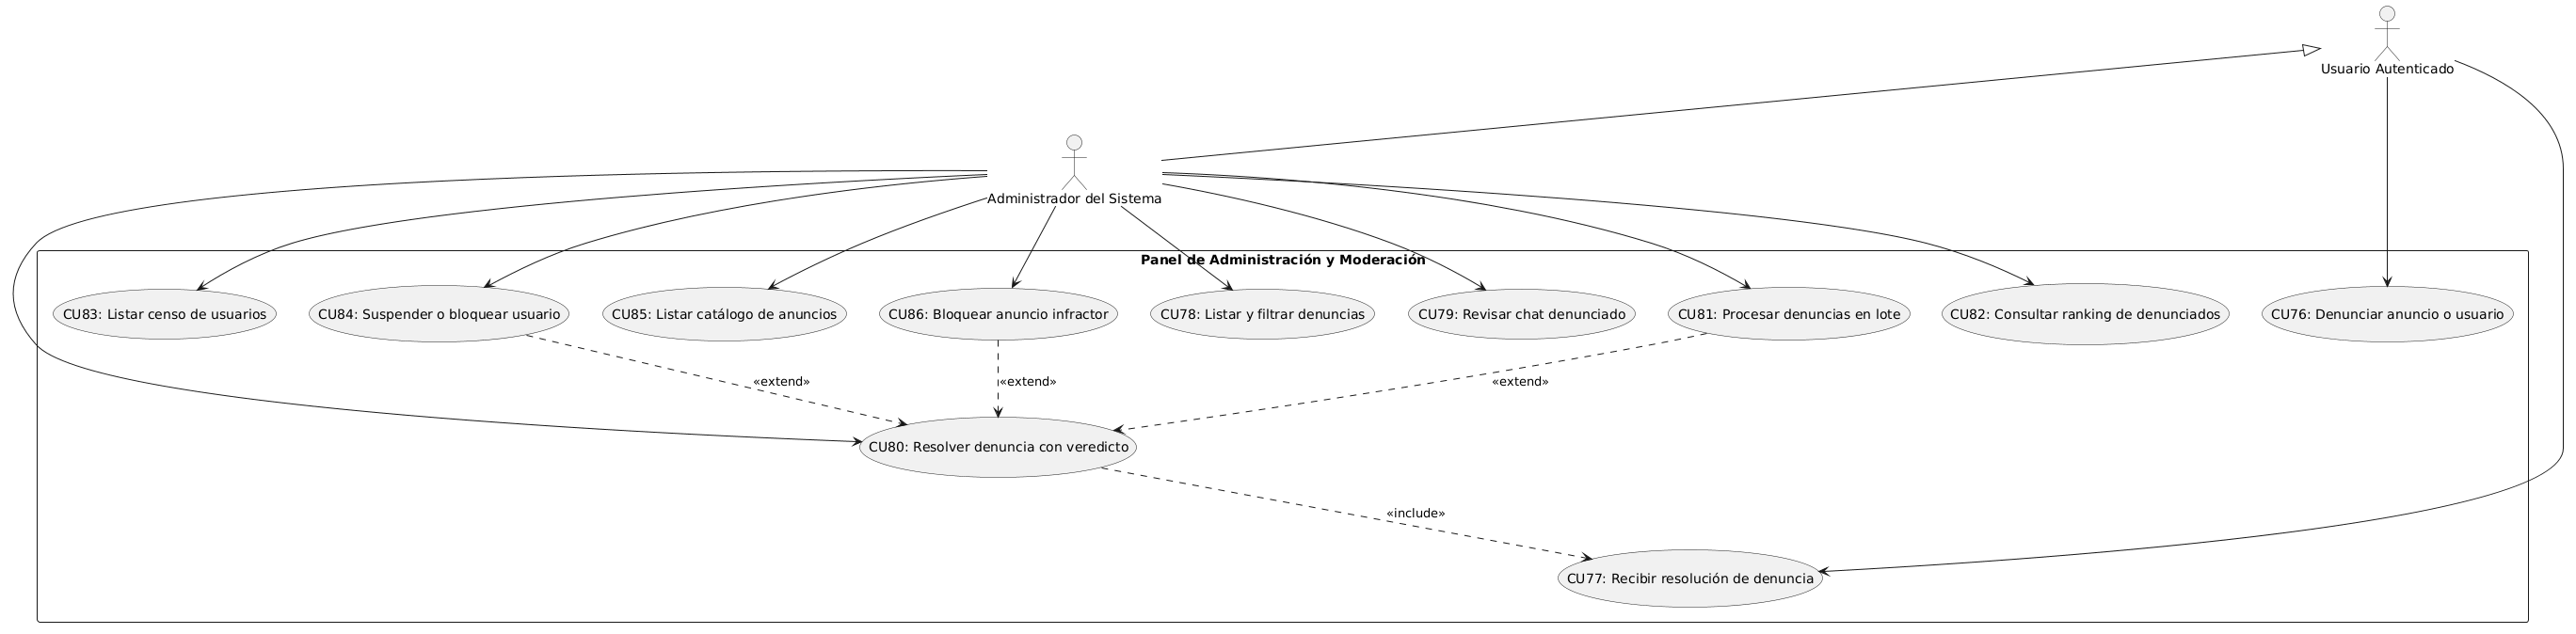
\includegraphics[width=0.88\textwidth]{AnalisisFuncional/img/dcu_moderacion.png}
    \caption{Diagrama de casos de uso de moderación y administración global}
    \label{fig:dcu_moderacion}
\end{figure}

    Las siguientes fichas estructuran las operaciones de moderación (CU76 a CU86):

\begin{table}[H]
\centering
\begin{tabular}{|p{3.2cm}|p{11.3cm}|}
\hline
\textbf{Caso de Uso} & \textbf{CU76: Denunciar anuncio, usuario o conversación} \\ \hline
\textbf{Actores} & Usuario Autenticado \\ \hline
\textbf{Descripción} & Remite una queja formal detallando una infracción sobre un contenido o conducta observada \\ \hline
\textbf{Precondiciones} & Estar autenticado y no haber denunciado previamente el mismo elemento si sigue en trámite \\ \hline
\textbf{Flujo básico} & 
1. El usuario pulsa sobre la opción de reporte presente en el anuncio, perfil o chat. \newline
2. El usuario selecciona la categoría del motivo y aporta una descripción justificativa. \newline
3. El backend registra la denuncia en estado pendiente dentro de la cola de moderación. \newline
4. El sistema confirma la recepción del reporte asignando un identificador de seguimiento. \\ \hline
\end{tabular}
\caption{Especificación del caso de uso CU76}
\label{tab:cu76}
\end{table}

\begin{table}[H]
\centering
\begin{tabular}{|p{3.2cm}|p{11.3cm}|}
\hline
\textbf{Caso de Uso} & \textbf{CU77: Recibir notificación de resolución de denuncia} \\ \hline
\textbf{Actores} & Usuario Autenticado \\ \hline
\textbf{Descripción} & Informa al usuario denunciante sobre el dictamen adoptado respecto a su notificación \\ \hline
\textbf{Precondiciones} & Haber interpuesto una denuncia que haya sido formalmente resuelta \\ \hline
\textbf{Flujo básico} & 
1. El sistema procesa el veredicto adoptado por el administrador sobre el expediente. \newline
2. El backend marca la denuncia con la confirmación de retroalimentación emitida. \newline
3. El sistema remite un aviso al panel de notificaciones del denunciante con el dictamen. \\ \hline
\end{tabular}
\caption{Especificación del caso de uso CU77}
\label{tab:cu77}
\end{table}

\begin{table}[H]
\centering
\begin{tabular}{|p{3.2cm}|p{11.3cm}|}
\hline
\textbf{Caso de Uso} & \textbf{CU78: Listar y filtrar cola global de denuncias} \\ \hline
\textbf{Actores} & Administrador del Sistema \\ \hline
\textbf{Descripción} & Despliega las quejas registradas permitiendo su clasificación por estado, severidad o tipo \\ \hline
\textbf{Precondiciones} & Disponer del rol de administración del sistema \\ \hline
\textbf{Flujo básico} & 
1. El administrador accede al panel de moderación global. \newline
2. El administrador aplica filtros por fecha, tipología del elemento o gravedad. \newline
3. El sistema recupera el listado paginado ordenado por orden cronológico y prioridad. \newline
4. La interfaz renderiza las tarjetas con el estado y los detalles preliminares del caso. \\ \hline
\end{tabular}
\caption{Especificación del caso de uso CU78}
\label{tab:cu78}
\end{table}

\begin{table}[H]
\centering
\begin{tabular}{|p{3.2cm}|p{11.3cm}|}
\hline
\textbf{Caso de Uso} & \textbf{CU79: Revisar historial de conversación denunciada} \\ \hline
\textbf{Actores} & Administrador del Sistema \\ \hline
\textbf{Descripción} & Audita de manera segura los mensajes intercambiados en un hilo objeto de investigación \\ \hline
\textbf{Precondiciones} & Que la denuncia corresponda formalmente a una infracción en el contexto del chat \\ \hline
\textbf{Flujo básico} & 
1. El administrador pulsa sobre el enlace de inspección dentro de la ficha del reporte. \newline
2. El sistema valida los permisos de auditoría y recupera los mensajes del canal. \newline
3. La interfaz presenta la secuencia íntegra de intervenciones para contrastar los hechos. \\ \hline
\end{tabular}
\caption{Especificación del caso de uso CU79}
\label{tab:cu79}
\end{table}

\begin{table}[H]
\centering
\begin{tabular}{|p{3.2cm}|p{11.3cm}|}
\hline
\textbf{Caso de Uso} & \textbf{CU80: Resolver denuncia individual con veredicto} \\ \hline
\textbf{Actores} & Administrador del Sistema \\ \hline
\textbf{Descripción} & Dictamina una queja asignando un estado de estimación o desestimación con notas técnicas \\ \hline
\textbf{Precondiciones} & Que el expediente de denuncia se encuentre en estado pendiente o en revisión \\ \hline
\textbf{Flujo básico} & 
1. El administrador introduce la justificación del veredicto y selecciona la resolución. \newline
2. El backend conmuta el estado de la denuncia a resuelta archivando el motivo del fallo. \newline
3. Se invoca de forma obligatoria la emisión de la notificación de retroalimentación al denunciante. \\ \hline
\end{tabular}
\caption{Especificación del caso de uso CU80}
\label{tab:cu80}
\end{table}

\begin{table}[H]
\centering
\begin{tabular}{|p{3.2cm}|p{11.3cm}|}
\hline
\textbf{Caso de Uso} & \textbf{CU81: Procesar denuncias en lote} \\ \hline
\textbf{Actores} & Administrador del Sistema \\ \hline
\textbf{Descripción} & Permite resolver conjuntamente múltiples denuncias vinculadas a un mismo infractor \\ \hline
\textbf{Precondiciones} & Existencia de al menos dos quejas pendientes asociadas a la misma entidad \\ \hline
\textbf{Flujo básico} & 
1. El administrador marca un grupo de denuncias acumuladas sobre un mismo elemento. \newline
2. El administrador define una resolución común y un veredicto unificado. \newline
3. Se extiende de forma reiterada la resolución individual con dictamen para cada expediente. \newline
4. El backend actualiza masivamente los registros dentro de una misma transacción. \\ \hline
\end{tabular}
\caption{Especificación del caso de uso CU81}
\label{tab:cu81}
\end{table}

\begin{table}[H]
\centering
\begin{tabular}{|p{3.2cm}|p{11.3cm}|}
\hline
\textbf{Caso de Uso} & \textbf{CU82: Consultar ranking de elementos más denunciados} \\ \hline
\textbf{Actores} & Administrador del Sistema \\ \hline
\textbf{Descripción} & Despliega métricas consolidadas sobre los usuarios y publicaciones con mayor tasa de reportes \\ \hline
\textbf{Precondiciones} & Disponer de credenciales activas de administrador \\ \hline
\textbf{Flujo básico} & 
1. El administrador accede al panel de métricas y tendencias de moderación. \newline
2. El sistema agrega la cantidad de reportes agrupados por identificador de entidad denunciada. \newline
3. La interfaz presenta una tabla ordenada descendentemente destacando a infractores recurrentes. \\ \hline
\end{tabular}
\caption{Especificación del caso de uso CU82}
\label{tab:cu82}
\end{table}

\begin{table}[H]
\centering
\begin{tabular}{|p{3.2cm}|p{11.3cm}|}
\hline
\textbf{Caso de Uso} & \textbf{CU83: Listar usuarios registrados con filtros} \\ \hline
\textbf{Actores} & Administrador del Sistema \\ \hline
\textbf{Descripción} & Muestra el censo global de cuentas en la plataforma permitiendo segmentar por estado o rol \\ \hline
\textbf{Precondiciones} & Estar autenticado con rol de administración \\ \hline
\textbf{Flujo básico} & 
1. El administrador entra en el módulo de gestión de usuarios del panel directivo. \newline
2. El administrador introduce un criterio de búsqueda como correo, nombre o estado disciplinario. \newline
3. El backend devuelve la lista paginada reflejando fechas de registro y avisos previos. \\ \hline
\end{tabular}
\caption{Especificación del caso de uso CU83}
\label{tab:cu83}
\end{table}

\begin{table}[H]
\centering
\begin{tabular}{|p{3.2cm}|p{11.3cm}|}
\hline
\textbf{Caso de Uso} & \textbf{CU84: Suspender o bloquear usuario de la plataforma} \\ \hline
\textbf{Actores} & Administrador del Sistema \\ \hline
\textbf{Descripción} & Inhabilita temporal o definitivamente el acceso al sistema de un infractor \\ \hline
\textbf{Precondiciones} & Que la cuenta a sancionar se encuentre actualmente en estado activo \\ \hline
\textbf{Flujo básico} & 
1. El administrador activa la sanción sobre el perfil del infractor especificando el motivo. \newline
2. Si la acción dimana de un informe disciplinario, se ejecuta de forma extendida sobre la resolución del reporte. \newline
3. El backend revoca de manera inmediata todos los tókenes JWT activos del usuario. \newline
4. El sistema bloquea los futuros intentos de autenticación impidiendo el acceso a la API. \\ \hline
\end{tabular}
\caption{Especificación del caso de uso CU84}
\label{tab:cu84}
\end{table}

\begin{table}[H]
\centering
\begin{tabular}{|p{3.2cm}|p{11.3cm}|}
\hline
\textbf{Caso de Uso} & \textbf{CU85: Listar catálogo global de anuncios} \\ \hline
\textbf{Actores} & Administrador del Sistema \\ \hline
\textbf{Descripción} & Examina la totalidad de los alojamientos registrados con independencia de su visibilidad \\ \hline
\textbf{Precondiciones} & Disponer de privilegios de administración \\ \hline
\textbf{Flujo básico} & 
1. El administrador accede a la auditoría del catálogo de propiedades. \newline
2. El sistema recupera los anuncios activos, pausados y bloqueados de todos los anfitriones. \newline
3. La interfaz permite consultar los importes, propietarios asociados e historiales de quejas. \\ \hline
\end{tabular}
\caption{Especificación del caso de uso CU85}
\label{tab:cu85}
\end{table}

\begin{table}[H]
\centering
\begin{tabular}{|p{3.2cm}|p{11.3cm}|}
\hline
\textbf{Caso de Uso} & \textbf{CU86: Bloquear o despublicar anuncio infractor} \\ \hline
\textbf{Actores} & Administrador del Sistema \\ \hline
\textbf{Descripción} & Retira una publicación del catálogo público por vulnerar las condiciones del servicio \\ \hline
\textbf{Precondiciones} & Que el anuncio figure en estado publicado o disponible \\ \hline
\textbf{Flujo básico} & 
1. El administrador selecciona la opción de bloqueo sobre la ficha del alojamiento infractor. \newline
2. Si procede de una denuncia, la medida se extiende sobre la resolución del reporte evaluado. \newline
3. El backend altera el estado de la publicación a bloqueada por moderación. \newline
4. El sistema purga la oferta de los resultados de búsqueda y del mapa interactivo. \\ \hline
\end{tabular}
\caption{Especificación del caso de uso CU86}
\label{tab:cu86}
\end{table}
